\documentclass[twocolumn,linenumbers]{aastex7}

% Paper 2 source for the multiphase galactic wind inference-validation project.
% All additions to this document should follow ../writing_style_guide.md.
% Keep generated figures, logs, and compiled PDF artifacts out of version control.
% Local compile check:
%   cd paper/paper2_inference_validation
%   TEXINPUTS=../aastex//: pdflatex -output-directory=/tmp/paper2_build paper2_inference_validation.tex

\shorttitle{Inference Validation for Multiphase Galactic Winds}
\shortauthors{Fielding et al.}

\begin{document}

\title{Validating Inference for Multiphase Galactic Wind Models}

\author{Drummond Fielding}
\affiliation{Center for Cosmology and Particle Physics, Department of Physics, New York University, New York, NY 10003, USA}
\email{TODO: add corresponding author email}

% \author{Coauthor Name}
% \affiliation{Coauthor Affiliation}

\begin{abstract}
% Outline:
% - Open with the central uncertainty: observations increasingly constrain cool outflow kinematics and columns, but it remains unclear which wind-launch and cloud-wind parameters can actually be inferred from those data.
% - State what this paper does: validates a Bayesian inference workflow for a multiphase analytic wind model before using it to interpret real absorption-line observations.
% - Name the method compactly: prior predictive checks, synthetic input recovery, posterior predictive checks, and sensitivity tests for turbulent radiative mixing-layer parameters.
% - State the baseline parameter set: hot mass loading, cold mass loading, and hot energy loading.
% - State the planned extension: test whether one effective cloud-wind interaction parameter is identifiable before adding more phenomenological knobs.
% - End with the implication: this gives a disciplined way to separate physically constrained wind properties from prior-dominated subgrid assumptions.
\end{abstract}

\keywords{galactic winds --- interstellar medium --- circumgalactic medium --- starburst galaxies --- Bayesian statistics}

\section{Introduction}
\label{sec:introduction}

% Outline:
% - Start from the astrophysical stakes: galactic winds regulate galaxy growth, metal transport, and circumgalactic gas, but the multiphase structure of those winds remains hard to infer.
% - Place Paper 1 in context: it connected the multiphase wind model to CLASSY-like observables but did not establish whether the fitted parameters were identifiable or robustly recoverable.
% - State the central problem for Paper 2: an inference pipeline can return posteriors even when the data do not actually constrain the requested physical parameters.
% - Introduce the validation logic: before fitting real systems, map the model's prior predictive behavior, recover known synthetic inputs, and only then ask whether deeper cloud-wind parameters can be fitted.
% - Preview the observational target: cool-phase absorption-line velocity distributions, especially moment summaries and binned dN/dv profiles.
% - End with a roadmap paragraph describing Sections \ref{sec:model}--\ref{sec:summary}.

\section{Forward Model and Observable Mapping}
\label{sec:model}

The forward model used in this paper is a steady, one-dimensional description of a starburst-driven multiphase wind.
It follows the classical picture in which supernovae and stellar winds thermalize inside a compact launch region and drive a hot, volume-filling outflow \citep{Chevalier85}.
The model then embeds cool clouds in this hot wind and evolves the two phases together as they exchange mass, momentum, and energy through turbulent, radiatively cooling interfaces \citep{Fielding22}.
The calculation is intentionally reduced: it does not attempt to resolve the cloud-wind interface directly, nor does it model the full three-dimensional geometry of a real outflow.
Instead, it asks whether a physically controlled radial model can map a small set of wind and cloud parameters into the cool-gas velocity and column-density distributions measured in absorption.

The main extension relative to the single-cloud implementation used in earlier applications is that the cool phase is represented by a mass spectrum.
The injected cool material is divided into logarithmically spaced cloud-mass bins, and each bin evolves as a separate cloud species with its own mass, velocity, metallicity, size, cooling parameter, and contribution to the final column-density profile.
This matters because small clouds are numerous and couple efficiently to the hot phase, while larger clouds can survive longer and carry substantial cold mass to larger radii.
The observable profile is therefore not the trajectory of one representative cloud, but the sum of many cloud species that respond differently to the same hot wind.
This section defines that forward map.
The statistical machinery used to fit or validate the model is introduced only after the physical model has been specified.

\subsection{Model Geometry and Hot-Wind Launch}
\label{subsec:model_launch}

We consider a radial wind subtending a solid angle $\Omega_{\rm wind}$.
The model is initialized at a characteristic launch radius $r_\star$, which should be interpreted as the radius at which the hot wind has passed through the sonic point and begins to interact with the cool cloud population followed in the calculation.
For a galaxy with star formation rate $\dot{M}_\star$, the hot phase is specified by two dimensionless loading factors.
The hot mass loading is
\begin{equation}
\dot{M}_{\rm hot} = \eta_M \dot{M}_\star ,
\end{equation}
and the hot energy injection rate is
\begin{equation}
\dot{E}_{\rm hot}
=
\eta_E
\frac{E_{\rm SN}}{m_\star}
\dot{M}_\star .
\end{equation}
Here $E_{\rm SN}$ is the mechanical energy per supernova and $m_\star$ is the stellar mass formed per supernova.
The ratio $\dot{E}_{\rm hot}/\dot{M}_{\rm hot}$ sets the specific energy of the hot wind, while $\eta_M$ and $\eta_E$ separately control the hot density, pressure, and cooling rate.

The launch state is set by imposing a Mach number slightly offset from unity,
\begin{equation}
{\cal M}_0 = 1 + \epsilon_{\rm sonic}.
\end{equation}
This small offset regularizes the transonic initial condition while keeping the solution tied to the sonic point.
In the current implementation the hot velocity at $r_\star$ is
\begin{equation}
v_\star =
\left(\frac{\dot{E}_{\rm hot}}{\dot{M}_{\rm hot}}\right)^{1/2}
\left[
\frac{1}{(\gamma-1){\cal M}_0}
+ \frac{1}{2}
\right]^{-1/2},
\end{equation}
with density fixed by mass-flux conservation,
\begin{equation}
\rho_\star =
\frac{\dot{M}_{\rm hot}}
{\Omega_{\rm wind} r_\star^2 v_\star},
\end{equation}
and pressure fixed by the Mach-number definition,
\begin{equation}
P_\star =
\frac{\rho_\star v_\star^2}{\gamma {\cal M}_0^2}.
\end{equation}
These equations are the implemented launch convention used by the calculations in this paper.
The same mass and energy injection rates also define source terms inside the launch region, normalized by the volume $4\pi r_\star^3/3$.
The flux normalization outside the launch region retains the explicit wind solid angle $\Omega_{\rm wind}$.

Gravity is represented by an isothermal potential,
\begin{equation}
\Phi(r) = v_{\rm circ}^2 \ln r ,
\end{equation}
where $v_{\rm circ}$ is the circular velocity of the galaxy.
Thus the fixed galaxy inputs that determine the hot-wind background are $\dot{M}_\star$, $r_\star$, $v_{\rm circ}$, and $\Omega_{\rm wind}$.
Increasing $\eta_E/\eta_M$ raises the specific energy and therefore the characteristic launch speed.
Increasing $\eta_M$ at fixed $\eta_E/\eta_M$ raises the hot density and makes radiative cooling and cloud coupling more important.
Changing $r_\star$ shifts the density scale through the area of the launch surface, while $v_{\rm circ}$ controls how strongly gravity decelerates the outflow.

\begin{figure*}[!htbp]
\centering
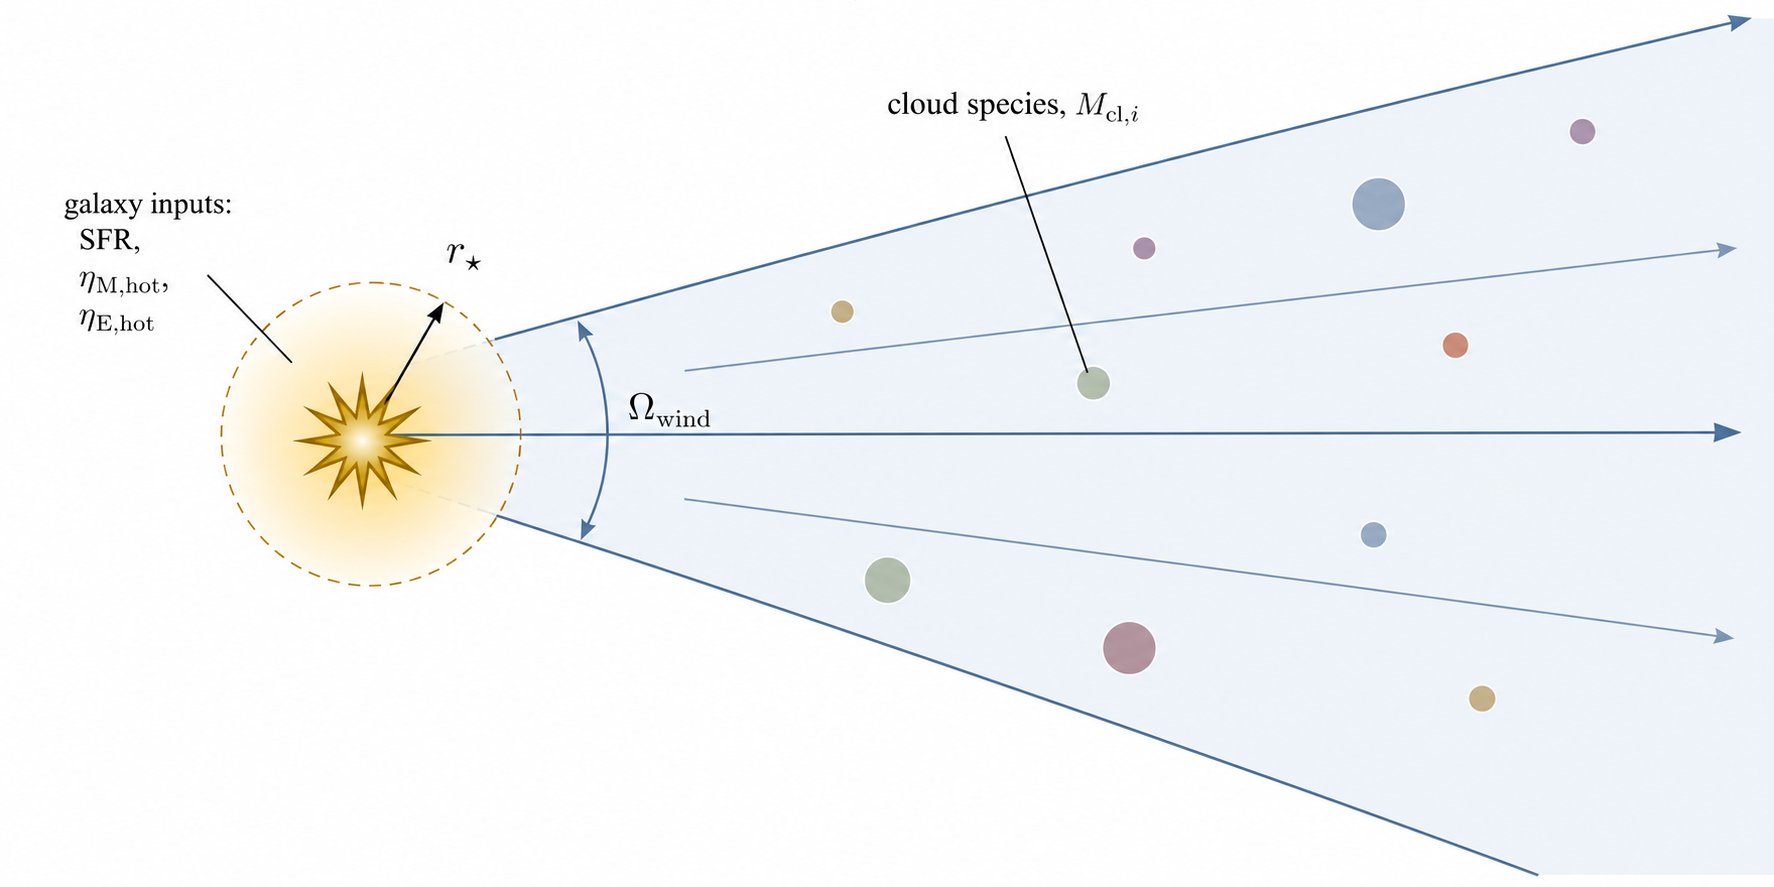
\includegraphics[width=0.92\textwidth]{figures/forward_model_launch_geometry.png}
\caption{
Conceptual geometry of the forward model launch region.
The hot wind is initialized at $r_\star$ after passing through the sonic point and then evolves radially through a straight biconical solid angle $\Omega_{\rm wind}$.
The launch region is set by the star formation rate and the hot mass and energy loading factors, while the colored circles indicate that the cool phase is represented by multiple cloud species with different initial masses.
This schematic is a guide to the implemented geometry and source terms, not a fit to any individual galaxy.
The numerical calculation is carried out in CGS units internally, while the user-facing quantities that set this launch problem include $\dot{M}_\star$, $\eta_{M,{\rm hot}}$, $\eta_{E,{\rm hot}}$, $r_\star$, and $\Omega_{\rm wind}$.
}
\label{fig:model_launch_geometry}
\end{figure*}

\subsection{Cold Cloud Mass Spectrum}
\label{subsec:model_cloud_spectrum}

The new ingredient in this paper is the explicit cloud mass spectrum.
Instead of choosing one representative cloud mass, we divide the injected cool phase into $N_{\rm cl}$ logarithmically spaced representative masses,
\begin{equation}
M_{{\rm cl},i}
=
10^{\log_{10}M_{\rm cl,min}+(i-1)\Delta\log_{10}M_{\rm cl}},
\end{equation}
where
\begin{equation}
\Delta\log_{10}M_{\rm cl}
=
\frac{\log_{10}M_{\rm cl,max}-\log_{10}M_{\rm cl,min}}{N_{\rm cl}-1}.
\end{equation}
These masses should be interpreted as species labels for a discretized cloud population, not as a claim that real clouds form at only these masses.
The continuous number injection spectrum is taken to be a power law,
\begin{equation}
\frac{d\dot{N}_{\rm cl}}{dM_{\rm cl}}
\propto
M_{\rm cl}^{-\alpha_{\rm cl}},
\end{equation}
or, equivalently,
\begin{equation}
\frac{d\dot{N}_{\rm cl}}{d\log_{10} M_{\rm cl}}
\propto
M_{\rm cl}^{1-\alpha_{\rm cl}}.
\end{equation}
The discrete relative number weight of species $i$ is therefore
\begin{equation}
w_{N,i}
=
M_{{\rm cl},i}^{1-\alpha_{\rm cl}}\Delta\log_{10} M_{\rm cl},
\end{equation}
up to an arbitrary normalization that cancels below.
The corresponding relative cold mass weight is
\begin{equation}
w_{M,i}
=
M_{{\rm cl},i}w_{N,i}.
\end{equation}

The total cold mass injection rate is set by a third loading factor,
\begin{equation}
\dot{M}_{\rm cold,tot}
=
\eta_{M,{\rm cold}}\dot{M}_\star .
\end{equation}
We assign this total flux to the discrete species according to the mass fraction
\begin{equation}
f_{M,i}
=
\frac{w_{M,i}}{\sum_j w_{M,j}},
\end{equation}
so that
\begin{equation}
\eta_{M,{\rm cold},i}
=
\eta_{M,{\rm cold}} f_{M,i},
\end{equation}
\begin{equation}
\dot{M}_{{\rm cold},i}
=
\eta_{M,{\rm cold},i}\dot{M}_\star ,
\end{equation}
\begin{equation}
\dot{N}_{{\rm cl},i}
=
\frac{\dot{M}_{{\rm cold},i}}{M_{{\rm cl},i}}.
\end{equation}
This construction separates the total amount of cold material, controlled by $\eta_{M,{\rm cold}}$, from how that material is divided among many cloud sizes, controlled by $\alpha_{\rm cl}$ and the cloud-mass bounds.
It also makes clear why $\alpha_{\rm cl}=2$ is a useful fiducial case.
For this slope, $w_{M,i}\propto M_{{\rm cl},i}^{2-\alpha_{\rm cl}}$ is approximately independent of mass, so each logarithmic mass interval receives a comparable share of the injected cold mass.
The number flux is very different: at fixed mass per logarithmic interval, the lowest-mass bins contain many more clouds.
This separation between mass weighting and number weighting is the central reason that a mass spectrum cannot usually be replaced by one effective cloud.
Figure~\ref{fig:cloud_mass_spectrum_initialization} shows this initialization for the fiducial spectrum used in the baseline inference tests.

\begin{figure*}[!htbp]
\centering
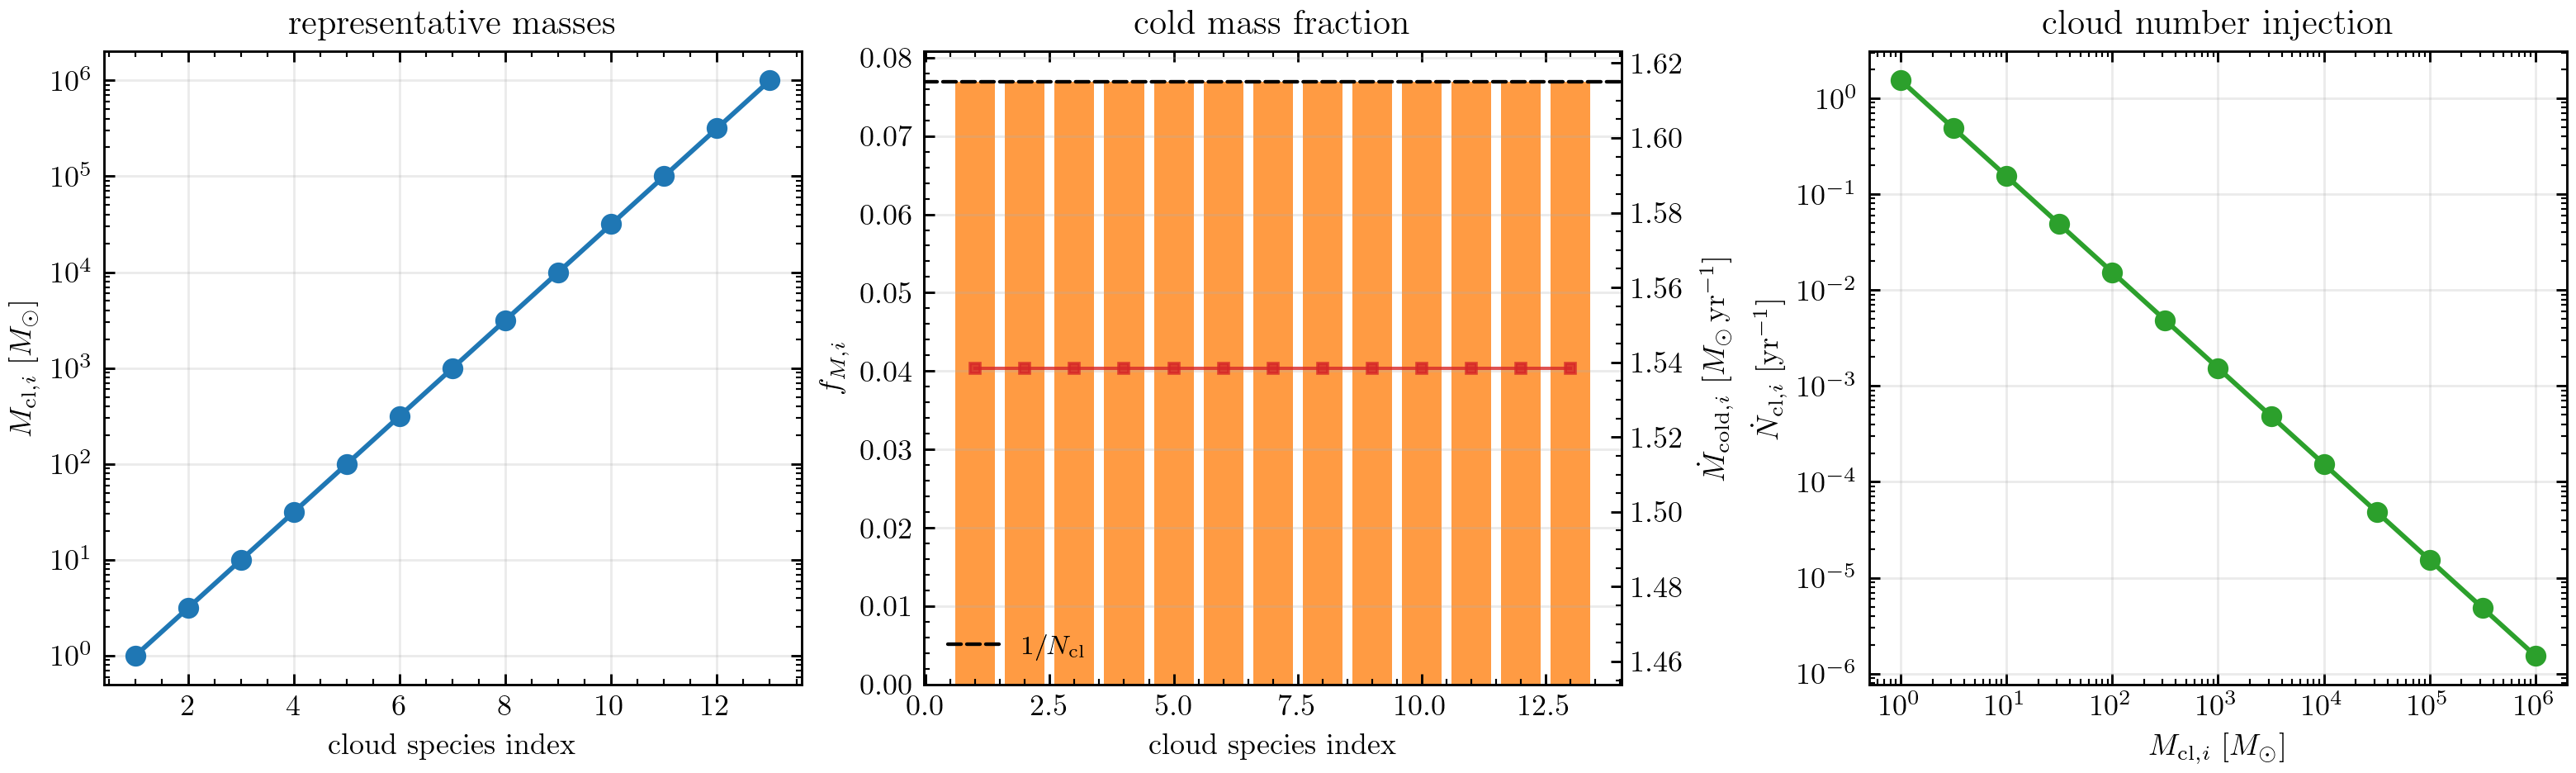
\includegraphics[width=\textwidth]{figures/cloud_mass_spectrum_initialization.png}
\caption{
Fiducial initialization of the cold cloud mass spectrum.
The representative masses span $M_{\rm cl,min}=1\,M_\odot$ to $M_{\rm cl,max}=10^6\,M_\odot$ with $N_{\rm cl}=13$ logarithmically spaced species.
For the default slope $\alpha_{\rm cl}=2$ and total cold mass loading $\eta_{M,{\rm cold}}=1$, the cold mass fraction is nearly flat across logarithmic mass bins, while the number injection rate falls approximately as $M_{\rm cl}^{-1}$.
Thus small clouds dominate the number budget even though they do not dominate the injected cold mass.
The plotted mass flux assumes $\dot{M}_\star=20\,M_\odot\,{\rm yr}^{-1}$.
}
\label{fig:cloud_mass_spectrum_initialization}
\end{figure*}

\subsection{Cloud Injection and Number Density}
\label{subsec:model_cloud_injection}

The quantities above define the asymptotic cloud number flux associated with each species.
In the implemented model, that flux is introduced over a finite radial interval rather than being switched on discontinuously at the launch radius.
Each cloud species has a radial number flux
\begin{equation}
\dot{N}_i(r)
=
\dot{N}_{i,0} I(r),
\end{equation}
where the injection profile is
\begin{equation}
I(r) =
\left\{
\begin{array}{ll}
\left(r/r_{\rm inj}\right)^{p_{\rm inj}}, & r < r_{\rm inj},\\
1, & r \ge r_{\rm inj}.
\end{array}
\right.
\end{equation}
The injection radius is tied to the hot-wind launch radius by
\begin{equation}
r_{\rm inj}
=
f_{\rm inj}r_\star .
\end{equation}
The current default values are $f_{\rm inj}=1.33$ and $p_{\rm inj}=6$.
This choice makes the cloud source term rise steeply just outside the launch region and reach its full value by $r_{\rm inj}$.
Flux conservation then gives the local number density of species $i$,
\begin{equation}
n_{{\rm cl},i}
=
\frac{\dot{N}_i(r)}
{\Omega_{\rm wind} r^2 v_{{\rm cl},i}}.
\end{equation}
The hot phase couples to the cold phase through sums over species of the form $n_{{\rm cl},i}\dot{M}_i$, $n_{{\rm cl},i}\dot{p}_i$, and $n_{{\rm cl},i}\dot{e}_i$.
This is where the mass spectrum matters dynamically.
The geometric factor $\Omega_{\rm wind}r^2$ dilutes all species in the same way, while the velocity factor accounts for residence time along the radial flow.
At fixed $v_{{\rm cl},i}$, species with larger $\dot{N}_{i,0}$ have larger number densities and therefore contribute more individual cloud interfaces per unit volume.
For the fiducial $\alpha_{\rm cl}=2$ initialization, this means that low-mass clouds can dominate the cloud count even when the cold mass density is initially distributed nearly evenly over logarithmic mass.
The subsequent evolution can then break this simple initialization because different masses accelerate, grow, and disrupt at different rates.
Figure~\ref{fig:cloud_injection_number_density} isolates the initialization effect before those dynamical differences appear.

\begin{figure}[!htbp]
\centering
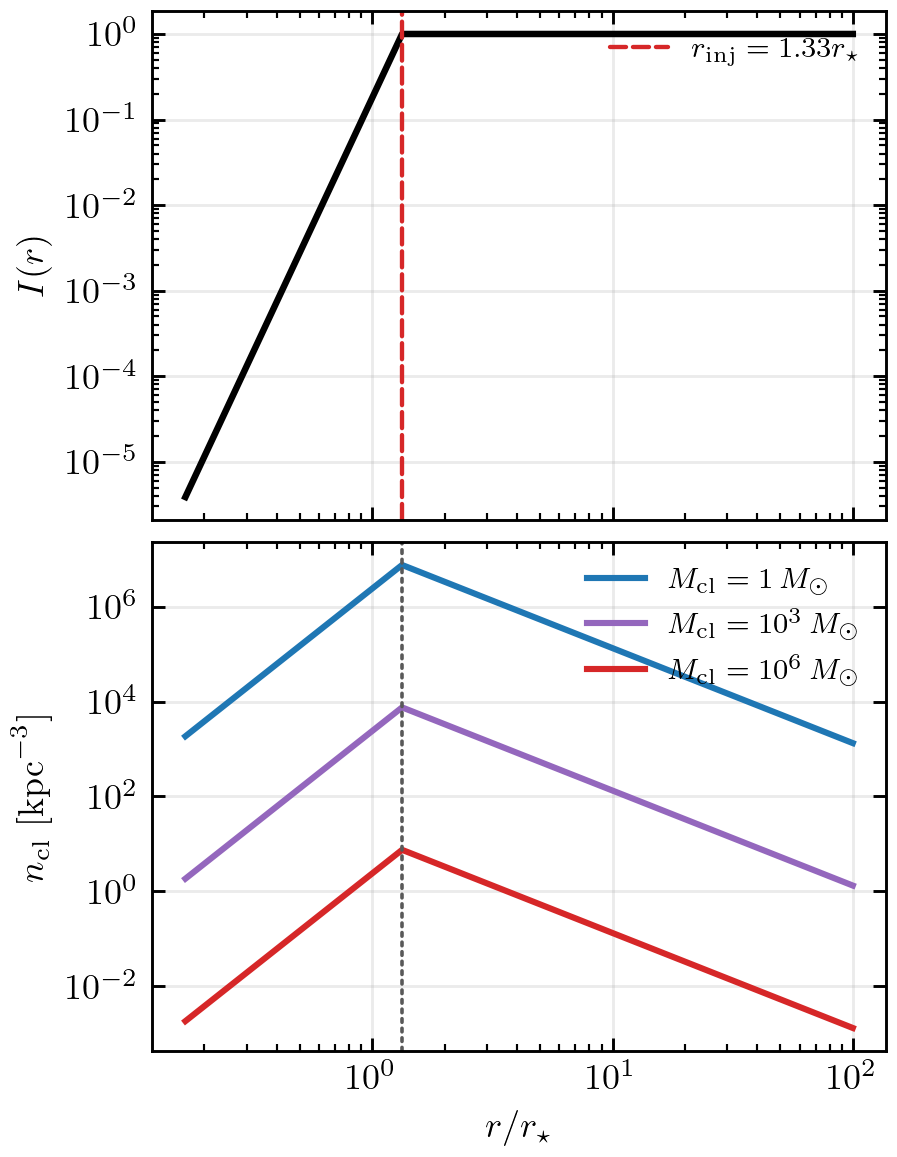
\includegraphics[width=\columnwidth]{figures/cloud_injection_number_density.png}
\caption{
Radial injection and initial number-density structure for the same fiducial cloud spectrum shown in Figure~\ref{fig:cloud_mass_spectrum_initialization}.
The top panel shows the implemented injection profile $I(r)$ with $r_{\rm inj}=1.33r_\star$ and $p_{\rm inj}=6$.
The bottom panel shows the corresponding cloud number density for three representative mass bins, assuming $r_\star=0.3\,{\rm kpc}$, $\Omega_{\rm wind}=4\pi$, and a common initial cloud velocity $v_{\rm cl,0}=100\,{\rm km}\,{\rm s}^{-1}$.
The number density is plotted in ${\rm kpc}^{-3}$ for readability.
The strong vertical separation between the curves is not a dynamical effect; it follows directly from distributing comparable cold mass over logarithmic bins while assigning much smaller masses to the low-mass species.
}
\label{fig:cloud_injection_number_density}
\end{figure}

\subsection{Pressure Equilibrium and Mixing-Layer Cooling}
\label{subsec:model_mixing_layer}

The cold clouds are assumed to remain in pressure equilibrium with the hot phase.
This is the closure that turns the hot-wind solution into cloud sizes, density contrasts, and cooling times.
For a fixed cloud temperature $T_{\rm cl}$,
\begin{equation}
\rho_{{\rm cl},i}
=
\frac{P\mu m_p}{k_B T_{\rm cl}},
\end{equation}
and
\begin{equation}
R_{{\rm cl},i}
=
\left(
\frac{3M_{{\rm cl},i}}
{4\pi \rho_{{\rm cl},i}}
\right)^{1/3}.
\end{equation}
The density contrast is
\begin{equation}
\chi_i =
\frac{\rho_{{\rm cl},i}}{\rho_{\rm hot}}.
\end{equation}
Because the cloud and hot phase are in pressure equilibrium, this density contrast is also approximately $T_{\rm hot}/T_{\rm cl}$.
The interface model is then controlled by the competition between turbulent mixing and radiative cooling.
The turbulent radiative mixing layer is evaluated at the geometric-mean temperature and metallicity,
\begin{equation}
T_{{\rm mix},i}
=
\left(T_{\rm hot}T_{\rm cl}\right)^{1/2},
\end{equation}
\begin{equation}
Z_{{\rm mix},i}
=
\left(Z_{\rm hot}Z_{{\rm cl},i}\right)^{1/2}.
\end{equation}
The relevant cooling time is
\begin{equation}
t_{{\rm cool},i}
=
t_{\rm cool}
\left(T_{{\rm mix},i},P/k_B,Z_{{\rm mix},i}/Z_\odot\right).
\end{equation}
Here the pressure argument is written as $P/k_B$ in units of ${\rm K}\,{\rm cm}^{-3}$, matching the cooling-table convention used in the code.
If the tabulated cooling function enters a net-heating regime, the implementation treats the interface cooling time as effectively long rather than allowing a negative cooling time to reverse the condensation prescription.

The turbulent velocity is modeled as
\begin{equation}
v_{{\rm turb},i}
=
f_{\rm turb}
\left|v_{\rm hot}-v_{{\rm cl},i}\right|
\chi_i^{a_{\rm turb}},
\end{equation}
which defines the cooling parameter
\begin{equation}
\xi_i
=
\frac{R_{{\rm cl},i}}
{v_{{\rm turb},i}t_{{\rm cool},i}}.
\end{equation}
The quantity $\xi_i$ compares the cloud radius to the distance a turbulent eddy travels in one mixed-layer cooling time.
It is therefore the most compact way to see which regime an interface occupies.
For $\xi_i \gtrsim 1$, mixed gas can cool before being advected away from the cloud surface, making condensation more effective.
For $\xi_i \lesssim 1$, the interface is more nearly mixing dominated and cloud destruction is favored.
The same hot wind can place different cloud masses in different regimes because $R_{{\rm cl},i}\propto M_i^{1/3}$ at fixed pressure.
Figure~\ref{fig:mixing_layer_cooling_parameter} shows this explicitly for the fiducial solved model used in the method figures.

\begin{figure}[!htbp]
\centering
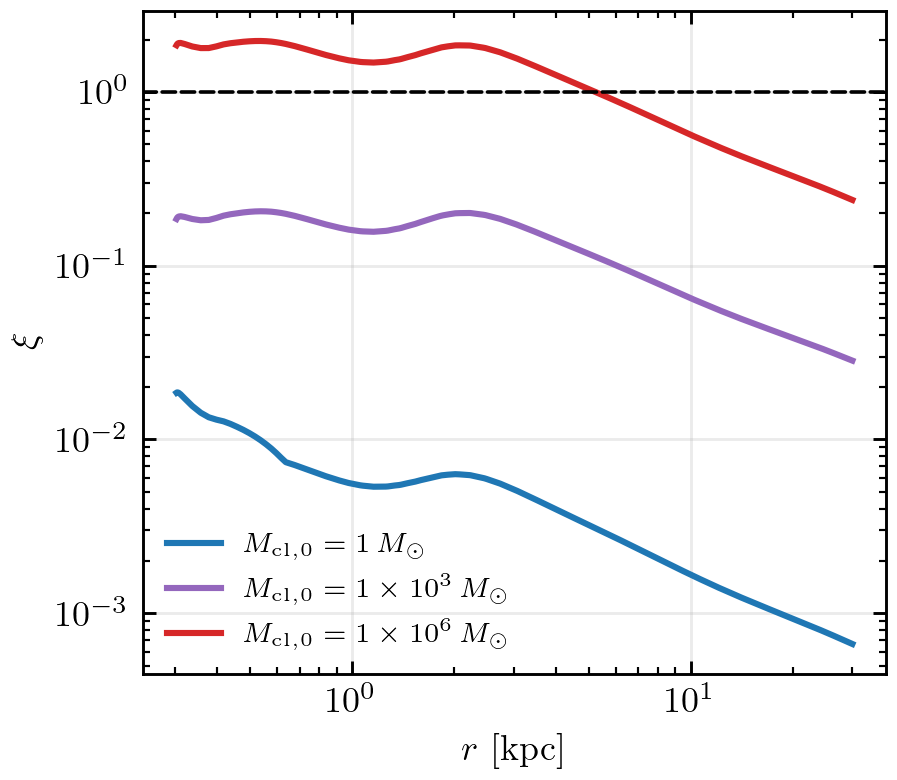
\includegraphics[width=\columnwidth]{figures/mixing_layer_cooling_parameter.png}
\caption{
Cooling parameter for three representative cloud species in the fiducial solved model.
The model uses $\dot{M}_\star=20\,M_\odot\,{\rm yr}^{-1}$, $v_{\rm circ}=150\,{\rm km}\,{\rm s}^{-1}$, $\eta_M=0.1$, $\eta_{M,{\rm cold}}=0.2$, $\eta_E=1$, and $r_\star=0.3\,{\rm kpc}$.
The dashed line marks $\xi=1$.
At fixed pressure, larger clouds have larger radii and therefore larger $\xi_i$, so they are closer to the radiatively efficient condensation regime than the low-mass species.
}
\label{fig:mixing_layer_cooling_parameter}
\end{figure}

\subsection{Cloud Mass Exchange}
\label{subsec:model_mass_exchange}

The model converts the cooling parameter into cloud growth and cloud loss rates.
For each active cloud species, the net cloud mass change is
\begin{equation}
\dot{M}_i =
\dot{M}_{{\rm grow},i}
+
\dot{M}_{{\rm loss},i}.
\end{equation}
The growth term is
\begin{equation}
\dot{M}_{{\rm grow},i}
=
C_M
\frac{3M_i v_{{\rm turb},i}}{R_i\chi_i}
A_i f_{\xi,i},
\end{equation}
where
\begin{equation}
A_i =
f_A \chi_i^{a_A},
\end{equation}
and
\begin{equation}
f_{\xi,i}
=
\left\{
\begin{array}{ll}
\xi_i^{1/2}, & \xi_i < 1,\\
\xi_i^{1/4}, & \xi_i \ge 1.
\end{array}
\right.
\end{equation}
The factor $A_i$ is an effective area enhancement for the turbulent interface, while $f_{\xi,i}$ encodes the change in condensation efficiency across the $\xi_i=1$ boundary.
The cloud mass-loss term is
\begin{equation}
\dot{M}_{{\rm loss},i}
=
-C_M
\frac{3M_i v_{{\rm turb,cold},i}}{R_i},
\end{equation}
with
\begin{equation}
v_{{\rm turb,cold},i}
=
v_{{\rm turb},i}\chi_i^{a_{\rm cold}}.
\end{equation}
These equations encode the central competition in the model.
Clouds grow when mixed gas cools rapidly enough to condense, and they lose mass when turbulent motions entrain cold gas into the hot flow faster than cooling can return it.
Clouds are removed from the active exchange terms once their mass falls below the implemented minimum cloud mass threshold.
This threshold prevents a numerically destroyed species from continuing to exert a spurious force through an arbitrarily small radius.

The important point for the mass-spectrum model is that the exchange rates do not scale linearly with cloud mass.
At fixed pressure, $R_i\propto M_i^{1/3}$, so the ratio $M_i/R_i$ scales as $M_i^{2/3}$, while the cooling parameter also grows as $M_i^{1/3}$.
Large clouds therefore have larger cooling parameters and longer survival times, but they are also less numerous at fixed total cold mass.
Small clouds present many interfaces to the hot wind and can couple strongly near the launch region, but they are more easily destroyed.
This is the physical reason that the multi-species model produces a distribution of cloud histories rather than a rescaled version of one trajectory.
Figure~\ref{fig:cloud_species_mass_velocity_evolution} shows the resulting divergence in mass survival and acceleration for representative species.

\begin{figure*}[!htbp]
\centering
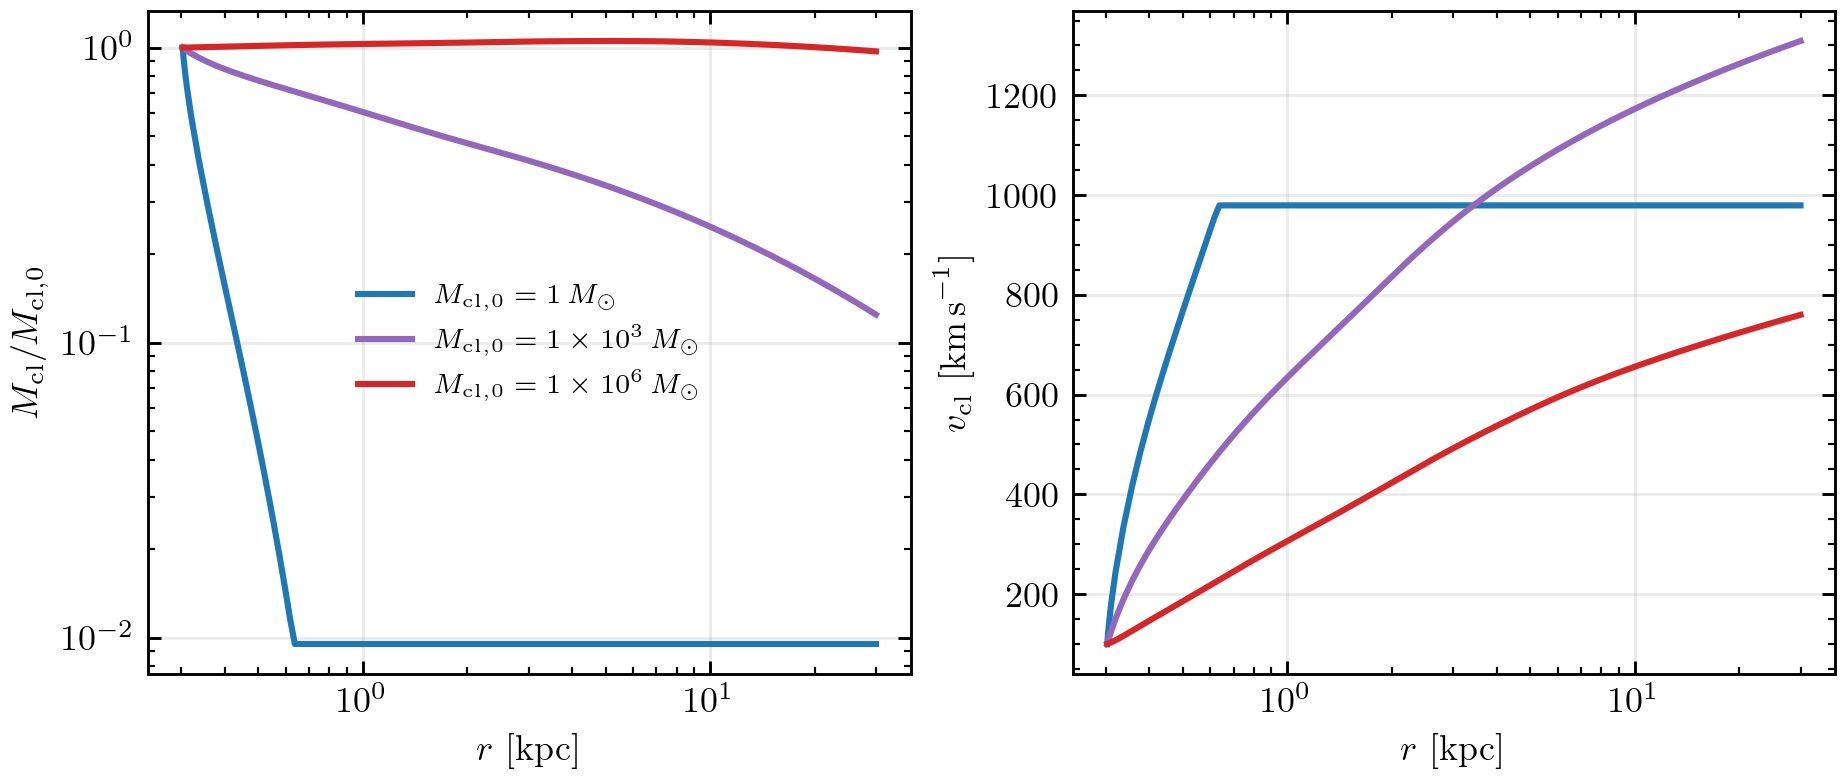
\includegraphics[width=0.78\textwidth]{figures/cloud_species_mass_velocity_evolution.png}
\caption{
Mass survival and acceleration of representative cloud species in the fiducial solved model.
The low-mass species has the smallest cooling parameter and is rapidly depleted, while the high-mass species survives to larger radius and accelerates more gradually.
The intermediate species illustrates that the transition between destruction and survival is continuous across the cloud mass spectrum.
These trajectories use the same fiducial parameters as Figure~\ref{fig:mixing_layer_cooling_parameter}; only three species are shown for clarity, but all thirteen species are included in the coupled wind calculation.
}
\label{fig:cloud_species_mass_velocity_evolution}
\end{figure*}

\subsection{Momentum and Energy Exchange}
\label{subsec:model_momentum_energy}

The mass exchange terms also carry momentum and energy.
The code treats two momentum channels separately: ram pressure on the cloud surface and the momentum advected by mass that changes phase.
The ram pressure force on species $i$ is
\begin{equation}
\dot{p}_{{\rm ram},i}
=
\frac{1}{2}C_D \rho_{\rm hot}
\pi R_i^2
v_{{\rm rel},i}\left|v_{{\rm rel},i}\right|,
\end{equation}
where $v_{{\rm rel},i}=v_{\rm hot}-v_i$.
With this convention, $\dot{p}_{{\rm ram},i}>0$ when the hot wind is faster than the cloud and the ram force accelerates the cloud outward.
The momentum carried by mass exchange is
\begin{equation}
\dot{p}_{{\rm trans},i}
=
v_{\rm hot}\dot{M}_{{\rm grow},i}
+
v_i\dot{M}_{{\rm loss},i}.
\end{equation}
The first term removes hot-wind momentum when hot or mixed material condenses onto the cloud.
The second term returns cloud material to the hot phase at the cloud velocity when $\dot{M}_{{\rm loss},i}<0$.

The hot phase also cools radiatively,
\begin{equation}
\dot{e}_{\rm cool}
=
-f_{\rm cool}
\left(\frac{\rho_{\rm hot}}{\mu_H m_p}\right)^2
\Lambda(P,\rho_{\rm hot},Z_{\rm hot}).
\end{equation}
The dimensionless factor $f_{\rm cool}$ is the implemented cooling multiplier; setting it to zero disables hot-phase radiative cooling, while values different from unity rescale the tabulated cooling loss.
The specific energy exchanged with cloud growth and destruction is written in terms of Bernoulli-like quantities,
\begin{equation}
B_{\rm hot}
=
\frac{1}{2}v_{\rm hot}^2
+
\frac{\gamma}{\gamma-1}\frac{P}{\rho_{\rm hot}}
+
\Phi,
\end{equation}
\begin{equation}
B_{{\rm cl},i}
=
\frac{1}{2}v_i^2
+
\frac{c_{s,{\rm cl}}^2}{\gamma-1}
+
\Phi.
\end{equation}
The cloud enthalpy term uses the cloud adiabatic sound speed $c_{s,{\rm cl}}^2=\gamma k_B T_{\rm cl}/(\mu m_p)$.
This convention follows the current implementation and avoids adding an extra factor of $\gamma$ to the cold thermal energy.
Thus
\begin{equation}
\dot{e}_{{\rm trans},i}
=
B_{\rm hot}\dot{M}_{{\rm grow},i}
+
B_{{\rm cl},i}\dot{M}_{{\rm loss},i}.
\end{equation}
The ram force also does work on the cloud at a rate that appears as a hot-phase sink proportional to $\dot{p}_{{\rm ram},i}v_{\rm hot}$ in the source terms below.

\subsection{Coupled Wind Equations}
\label{subsec:model_coupled_equations}

The hot wind is evolved with source terms from supernova injection, radiative cooling, gravity, and all cloud species.
The full steady equations are written in conservative form and then rearranged into radial derivatives for the variables integrated by the solver.
For interpreting the signs, it is useful to define the local source densities that enter the hot-phase mass, momentum, and energy budgets:
\begin{equation}
S_\rho
=
q_M
-
\sum_i n_i \dot{M}_i,
\label{eq:hot_mass_source}
\end{equation}
\begin{equation}
S_p
=
-
\sum_i n_i
\left(
\dot{p}_{{\rm trans},i}
+
\dot{p}_{{\rm ram},i}
\right),
\label{eq:hot_momentum_source}
\end{equation}
\begin{equation}
S_e
=
q_E
-
\sum_i n_i
\left(
\dot{e}_{{\rm trans},i}
+
\dot{p}_{{\rm ram},i}v_{\rm hot}
\right)
+
\dot{e}_{\rm cool}.
\label{eq:hot_energy_source}
\end{equation}
Here $q_M$ and $q_E$ are the hot mass and energy injection rates per unit volume inside the launch region.
The signs are chosen from the point of view of the hot phase.
A positive cloud mass growth rate, $\dot{M}_i>0$, removes mass from the hot phase and therefore contributes negatively to $S_\rho$.
A positive ram force accelerates the cloud and removes hot-wind momentum, giving a negative contribution to $S_p$.
Because $\dot{e}_{\rm cool}<0$, radiative cooling is always an energy sink for the hot phase when the cooling multiplier is positive.

These source terms are multiplied by the local cloud number density before being summed.
Consequently, a species can matter dynamically either because each cloud exchanges mass, momentum, or energy rapidly, or because the species contains many clouds per unit volume.
The latter route is especially important for the low-mass end of the spectrum.
The full numerical integration evolves the hot variables together with $M_i(r)$, $v_i(r)$, and $Z_i(r)$ for every cloud species.
Figure~\ref{fig:cloud_coupling_source_terms} shows the signed cloud back-reaction source terms in the fiducial model.

\begin{figure*}[!htbp]
\centering
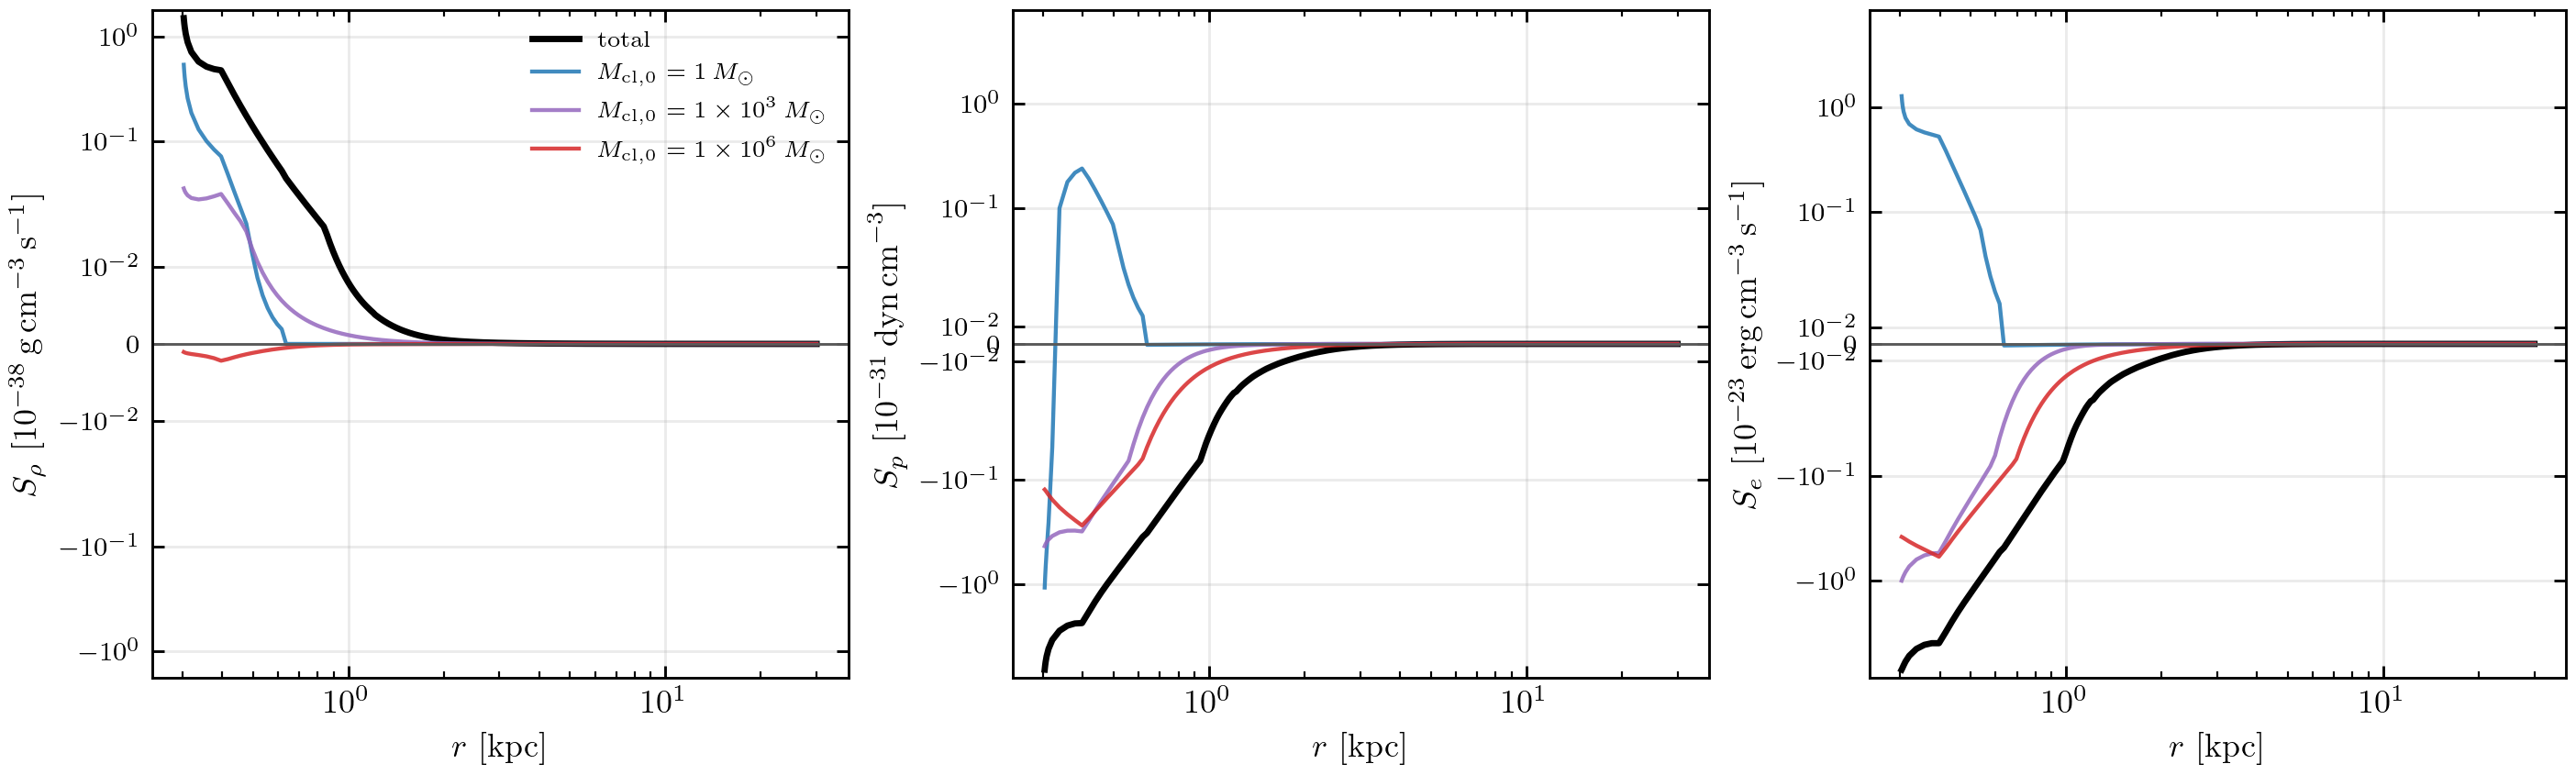
\includegraphics[width=\textwidth]{figures/cloud_coupling_source_terms.png}
\caption{
Signed cloud back-reaction source terms for the fiducial solved model.
The panels show the cloud contribution to the hot-phase mass, momentum, and energy source densities, following the sign conventions in Equations~(\ref{eq:hot_mass_source})--(\ref{eq:hot_energy_source}) but omitting the direct supernova source terms and hot radiative cooling term.
Each y-axis is scaled by the power of ten shown in its label.
Positive values add the corresponding conserved quantity to the hot phase, while negative values remove it.
The black curve is the sum over all cloud species; colored curves show representative low-, intermediate-, and high-mass species.
}
\label{fig:cloud_coupling_source_terms}
\end{figure*}

\subsection{Column-Density Velocity Profiles}
\label{subsec:model_observables}

The primary observable predicted by the model is the cool-gas column-density velocity distribution.
This is the step that connects the radial cloud trajectories to absorption-line data.
For cloud species $i$, the cold mass density along the flow is
\begin{equation}
\rho_{{\rm cold},i}
=
\frac{\dot{N}_i M_i}
{\Omega_{\rm wind}r^2v_i},
\end{equation}
and the corresponding hydrogen number density is
\begin{equation}
n_{{\rm H},i}
=
\frac{\rho_{{\rm cold},i}}{\mu_{\rm cool}m_p}.
\end{equation}
For monotonic cloud velocity histories,
\begin{equation}
\frac{dN}{dv}
\simeq
\sum_i
\frac{n_{{\rm H},i}}{\left|dv_i/dr\right|}.
\end{equation}
Only active cloud segments contribute to this transform.
If a species has been destroyed, it should not continue to add column at its final numerical velocity.
In practice, the observable calculation evaluates each species on the model radial grid, removes inactive segments, and interpolates the resulting contribution onto a common velocity grid before summing over species.
This species-resolved treatment is important because different initial cloud masses populate different velocity ranges.

For the binned observable used later in the paper, we instead compute a kernel-smoothed profile,
\begin{equation}
\left(\frac{dN}{dv}\right)_k
=
\sum_i
\int
n_{{\rm H},i}(r)
K_\sigma\left[v_i(r)-v_k\right]\,dr .
\end{equation}
Velocity moments and compact shape summaries are computed from this same profile.
The total column-density profile is therefore not determined by a single cloud acceleration history.
It is a weighted sum over survival, acceleration, and number density across the full cloud mass spectrum.
Figure~\ref{fig:cloud_species_dndv_contributions} shows this decomposition for the fiducial model.
The inference machinery introduced below operates on these predicted observable summaries rather than directly on the internal cloud trajectories.

\begin{figure}[!htbp]
\centering
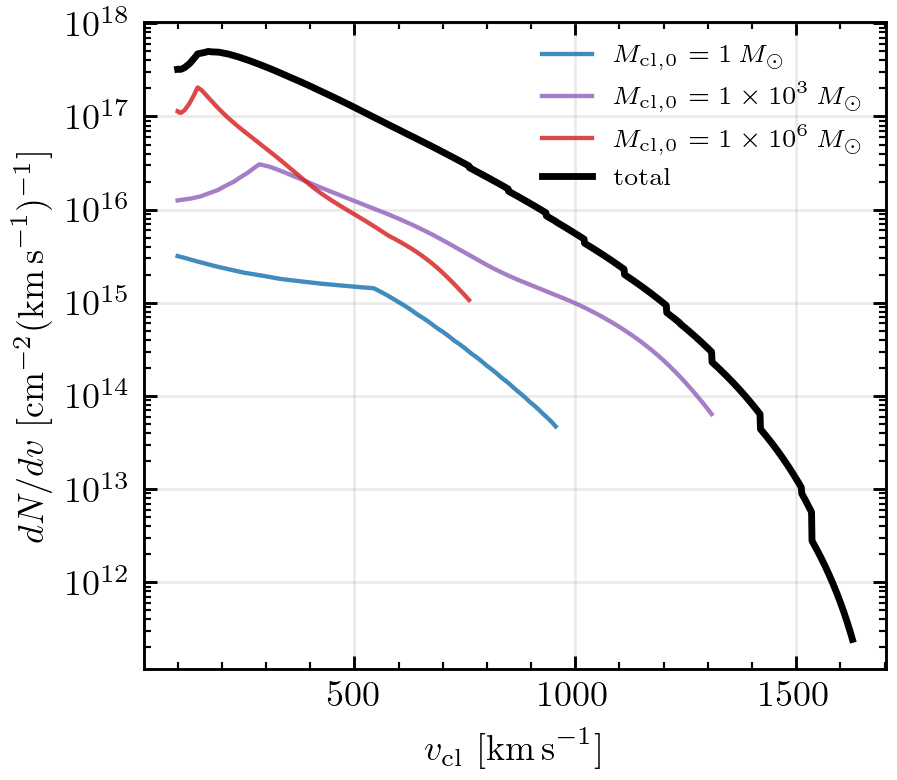
\includegraphics[width=\columnwidth]{figures/cloud_species_dndv_contributions.png}
\caption{
Species-resolved contribution to the cool-gas column-density velocity profile for the fiducial solved model.
The black curve is the total $dN/dv$ summed over all active cloud species.
The colored curves show representative low-, intermediate-, and high-mass species.
The low-mass species contributes at relatively low column because it is rapidly depleted, while the longer-lived species populate the higher-velocity part of the profile.
This decomposition is the observable counterpart of the mass and velocity histories in Figure~\ref{fig:cloud_species_mass_velocity_evolution}.
}
\label{fig:cloud_species_dndv_contributions}
\end{figure}

\section{Inference Framework}
\label{sec:inference_framework}

% Outline:
% - Explain inference in forward-model language: parameters map to observables, and the likelihood measures agreement with data.
% - Define priors, likelihoods, posteriors, and posterior predictive checks in physics terms.
% - Specify the baseline likelihood assumptions and covariance choices.
% - Describe MAP and posterior sampling only as much as needed to interpret the validation tests.
% - Make the key point: the goal is not to fit as many parameters as possible, but to learn which physical degrees of freedom are identifiable.

\section{Prior Predictive Checks}
\label{sec:prior_predictive}

% Outline:
% - State the question: what range of observables does the model produce before seeing data?
% - Describe the baseline prior ranges for eta_M, eta_M,cold, and eta_E.
% - Show the valid/failure fraction and where failures occur in parameter space.
% - Present distributions of column scale, mean velocity, velocity width, and profile shape.
% - Compare the prior predictive envelope to the scale of CLASSY-like observations.
% - Use this section to motivate any narrowing of priors before synthetic recovery.
% - End with a clear decision: whether the baseline prior is scientifically useful enough for input recovery.

\begin{figure*}[t]
\centering
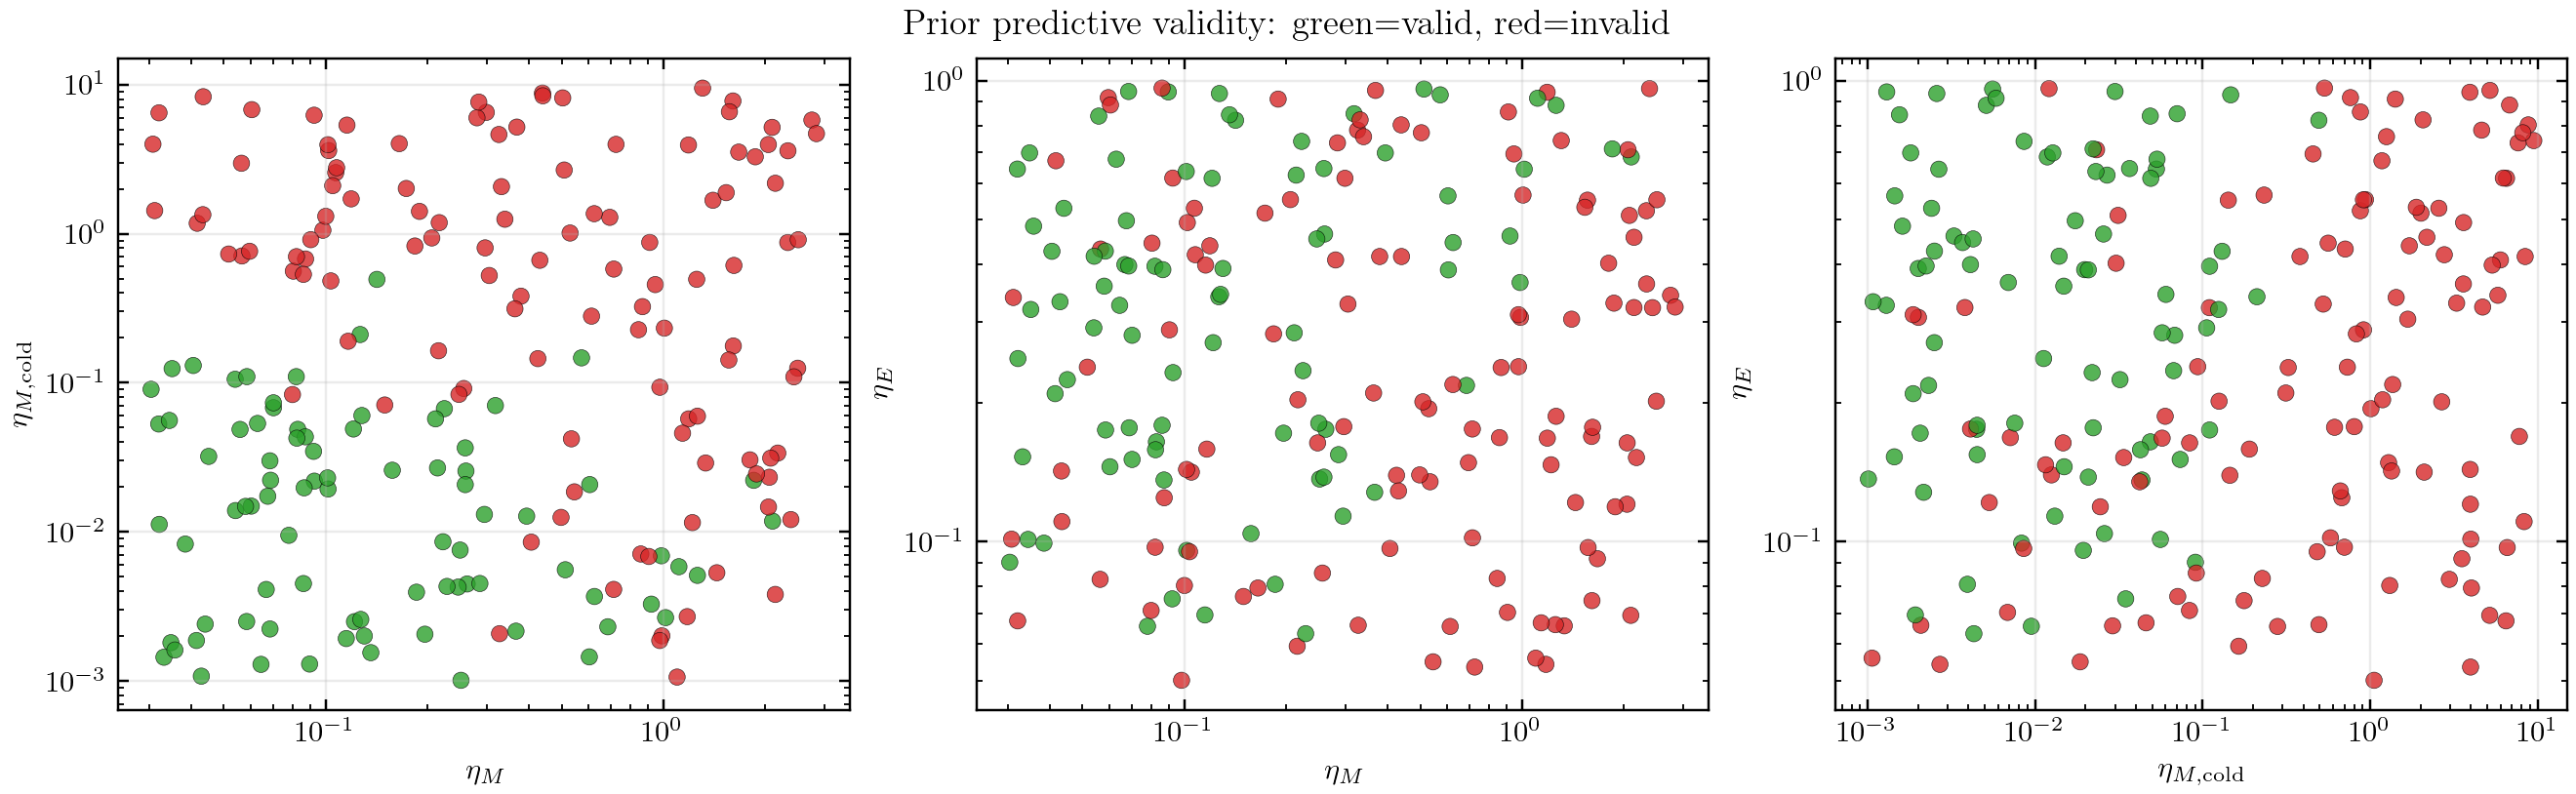
\includegraphics[width=\textwidth]{figures/prior_predictive_validity.png}
\caption{
Preliminary prior predictive validity map for the baseline three-parameter inference model.
The samples are drawn from broad exploratory priors on the hot mass loading, cold mass loading, and hot energy loading.
Green points mark parameter combinations that produce finite, physically valid observables, while red points mark failed integrations or invalid observable vectors.
This figure is meant to identify where the prior places probability on physically useful winds before any comparison with data.
}
\label{fig:prior_predictive_validity}
\end{figure*}

\begin{figure*}[t]
\centering
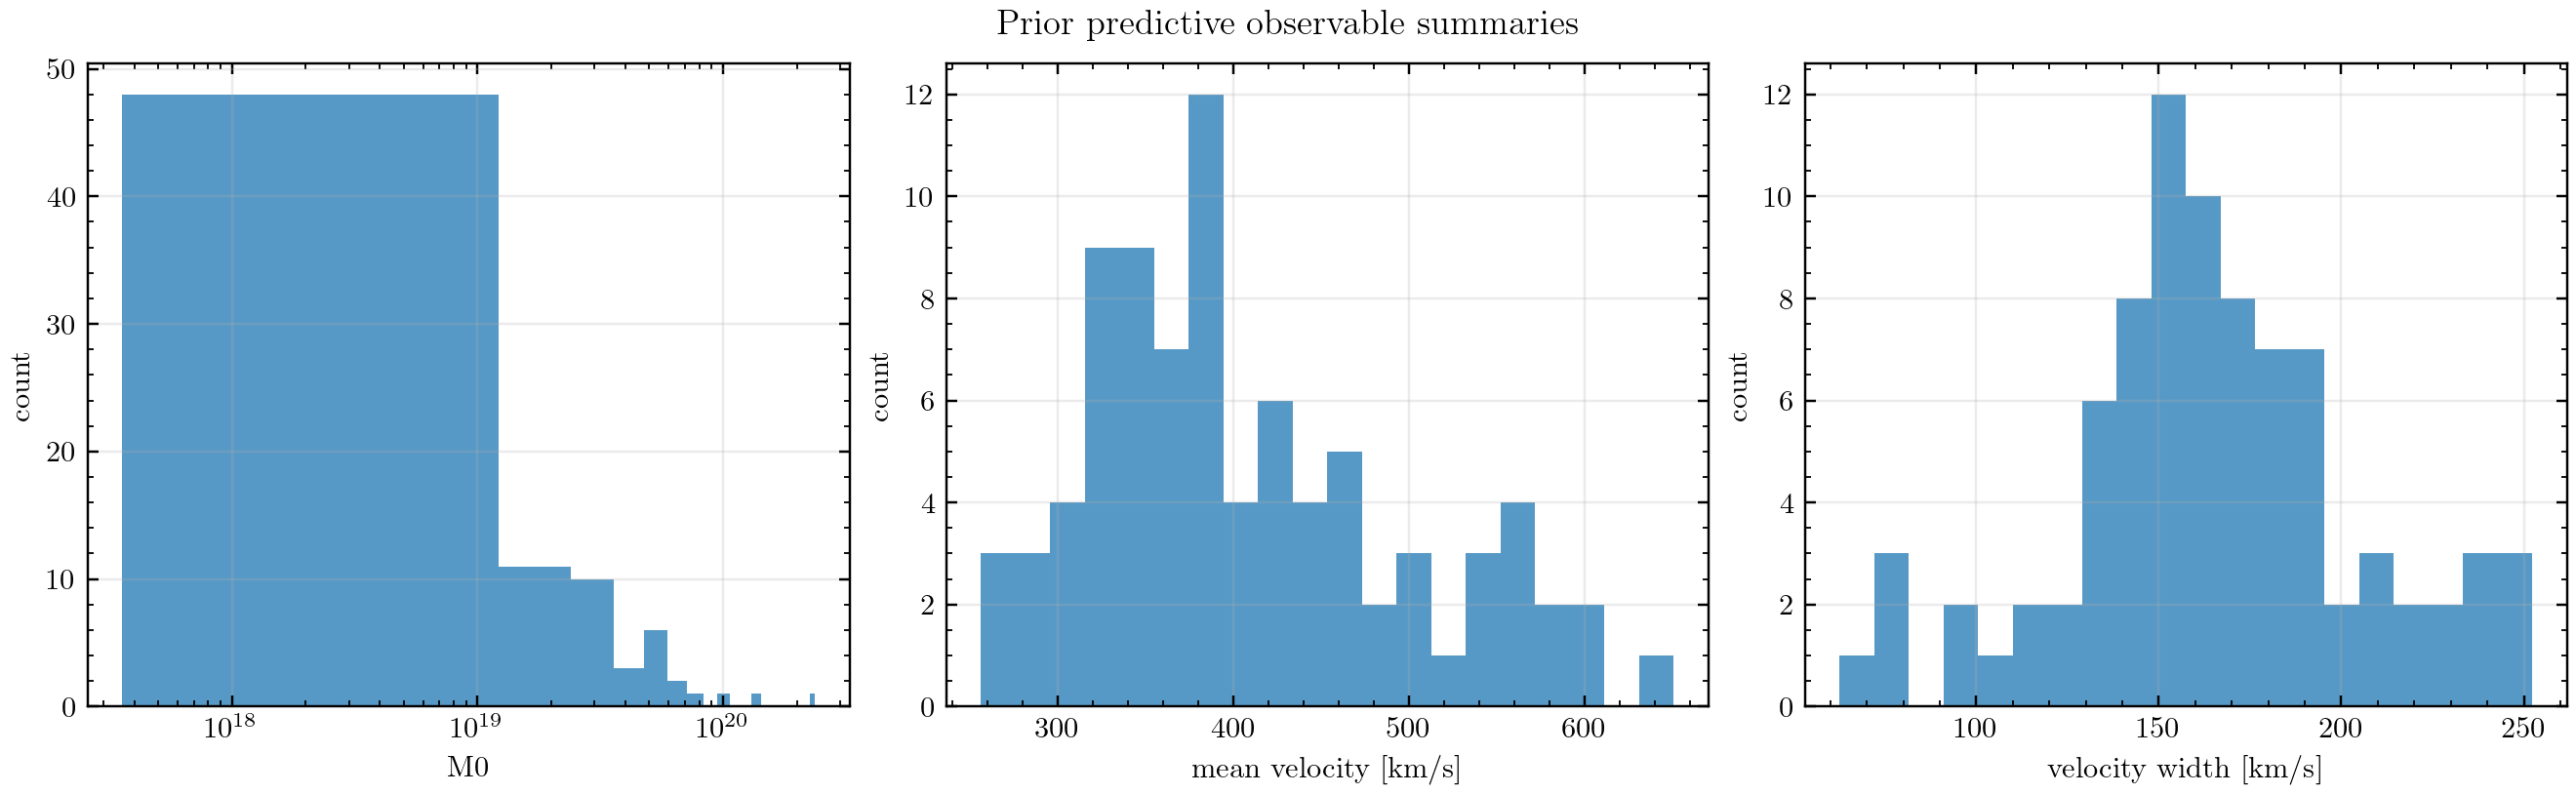
\includegraphics[width=\textwidth]{figures/prior_predictive_observable_histograms.png}
\caption{
Preliminary prior predictive distributions for three compact observable summaries computed from valid baseline samples.
The panels show the total column scale, mean velocity, and velocity width implied by the broad exploratory prior.
These distributions define the range of cool-phase absorption signatures that the current model expects before seeing the data, and therefore set the scale for the synthetic recovery tests that follow.
}
\label{fig:prior_predictive_observable_histograms}
\end{figure*}

\begin{figure*}[t]
\centering
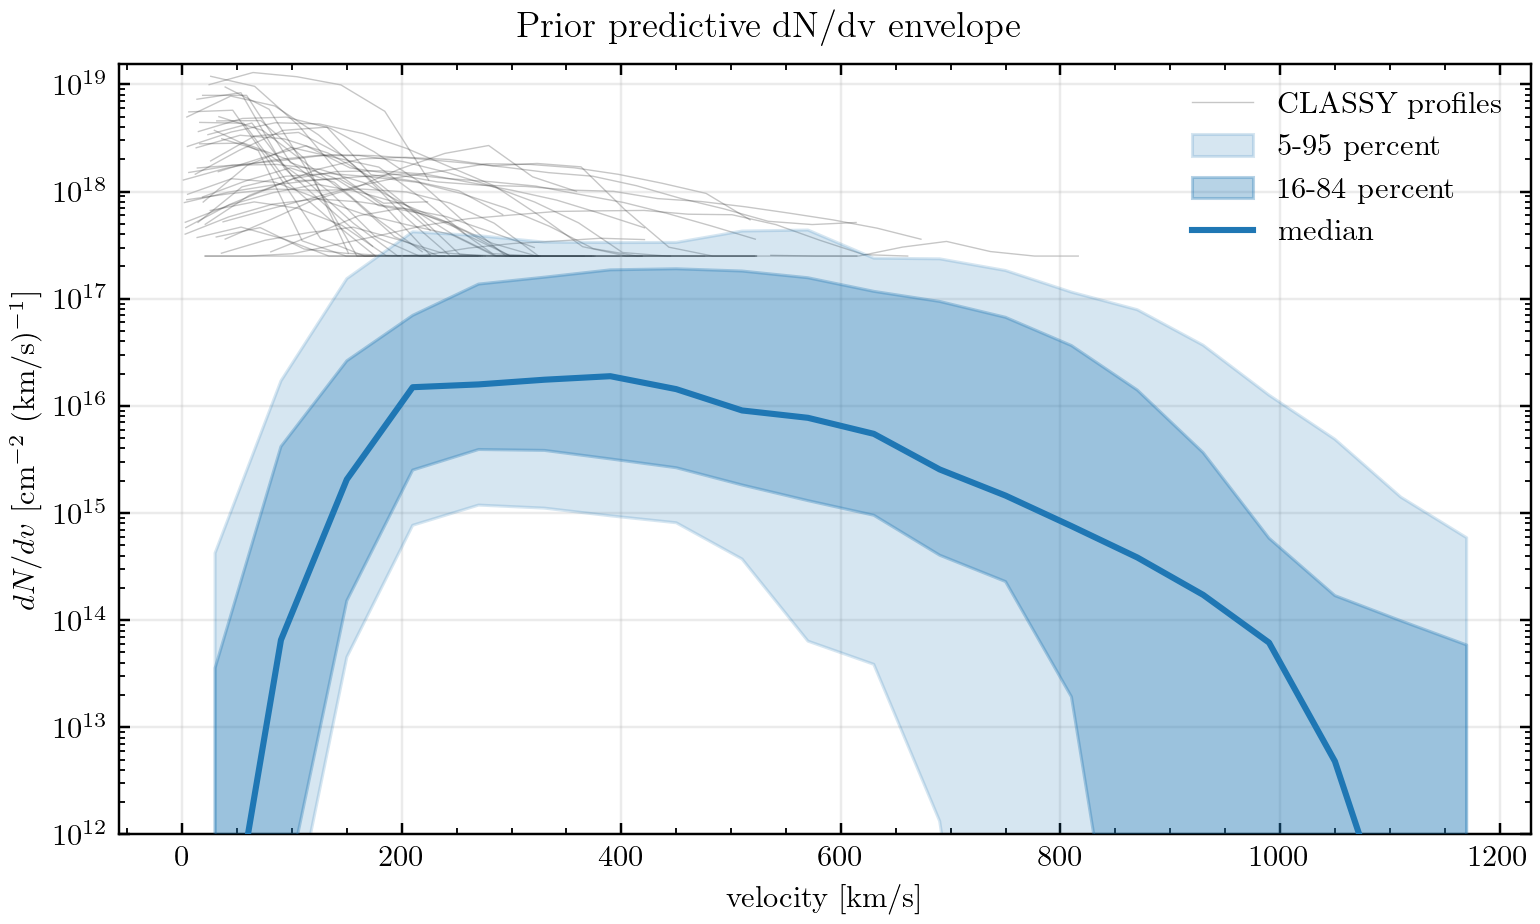
\includegraphics[width=0.82\textwidth]{figures/prior_predictive_dndv_envelope.png}
\caption{
Preliminary prior predictive envelope for the binned column-density velocity profile.
Thin gray curves show the processed CLASSY profiles after mapping blueshifted velocities to positive outflow speeds.
The shaded regions show the central prior-predictive spread among valid samples, and the solid blue curve shows the median model profile.
This comparison is intentionally imperfect: the blue prior predictive distribution is evaluated for one fixed fiducial galaxy with $\mathrm{SFR}=20\,M_\odot\,\mathrm{yr}^{-1}$, $r_\star=0.3\,\mathrm{kpc}$, and $v_{\rm circ}=150\,\mathrm{km}\,\mathrm{s}^{-1}$, while the gray curves span the full CLASSY sample with different galaxy properties.
The apparent vertical offset should therefore be read as a warning about this non-conditioned prior check, not as evidence that the model cannot fit individual CLASSY profiles.
The lower plotting limit is set to $10^{12}\,\mathrm{cm}^{-2}\,(\mathrm{km}\,\mathrm{s}^{-1})^{-1}$ to show the low-column prior tails without extending to the numerical floor used for model bookkeeping.
This profile-level check complements the moment-based summaries in Figure~\ref{fig:prior_predictive_observable_histograms} by asking whether the prior generates plausible velocity structure rather than only plausible low-order moments.
}
\label{fig:prior_predictive_dndv_envelope}
\end{figure*}

\section{Synthetic Input Recovery}
\label{sec:synthetic_recovery}

% Outline:
% - State the question: if we generate fake data from known wind parameters, can the inference recover them?
% - Define the baseline truth cases used by examples/inference_synthetic_recovery.py:
%   fiducial, low_eta_m_high_eta_e, high_eta_m_low_eta_e, low_eta_m_cold,
%   high_eta_m_cold, near_failure_boundary, strong_wings, and narrow_profile.
% - Use the same three observable modes as the inference code: raw M0-M2 moments,
%   logM0/mean/sigma/skewness/kurtosis, and binned dN/dv.
% - Define the synthetic covariance model explicitly: correlated fractional errors
%   for raw moments, mixed fractional/absolute errors for the transformed shape
%   moments, and AR(1) bin-to-bin covariance with a profile-amplitude floor for dN/dv.
% - Present recovery metrics: truth coverage in 68 and 95 percent intervals, posterior
%   mean and median bias, posterior width, MAP error, chi-square, sampler acceptance,
%   divergences, R-hat, ESS, and the parameter correlation matrix.
% - Compare raw moments, shape-five observables, and binned dN/dv.
% - Identify the dominant degeneracies among eta_M, eta_M,cold, and eta_E.
% - Close by stating whether the baseline three-parameter inference is trustworthy enough to apply to real data or extend.

\section{Sensitivity to Cloud-Wind Microphysics}
\label{sec:microphysics_sensitivity}

The synthetic recovery tests above motivate a deliberately modest next step.
Rather than fitting additional cloud-wind or turbulent radiative mixing-layer
parameters immediately, we first vary each fixed parameter one at a time and
measure how strongly the predicted observables respond.  This separates two
questions that are otherwise easy to confuse.  A microphysical parameter may be
important for the wind solution, but still be difficult to infer if its
observable effect is nearly parallel to a change in $\eta_M$,
$\eta_{M,\rm cold}$, or $\eta_E$.

We therefore treat the sensitivity screen as a forward-model diagnostic, not as
a larger posterior model.  The fitted parameter set remains the three loading
parameters.  Around each synthetic truth case, we vary one fixed cloud-wind
parameter at a time and compare the resulting observables with the baseline
prediction.  The screen includes the turbulent velocity normalization
$f_{\rm turb}$, drag coefficient $C_D$, mass-exchange prefactor, geometric area
factor, cloud mass-spectrum slope, metallicities, hot cooling multiplier, and
the $\chi$-dependent exponents that control the turbulent velocity and cooling
area scalings.  The same reduced CPU settings used in the exact recovery tests
are used here: $r_{\rm max}=6\,{\rm kpc}$, $\Delta r=0.08\,{\rm kpc}$, four
cloud-mass species, and cloud masses from $10$ to $10^4\,M_\odot$.

The screen is run in three stages.  First, all fixed parameters are scanned for
the five compact shape observables used in the baseline recovery tests.  Second,
the strongest and most physically plausible candidates are scanned in the
observed-window $\log dN/dv$ likelihood over $100$--$600\,{\rm km\,s^{-1}}$,
with the same low-signal censoring used in the final \texttt{strong\_wings}
diagnostic.  Third, the stable mixing-amplitude shortlist is checked with the
linear binned $dN/dv$ profile over the same velocity window.  For every scan
point we record the validity status, stalled-wind diagnostics, shifts in
shape summaries, profile distances, and a covariance-whitened projection of
the microphysics observable displacement onto the local subspace spanned by
finite-difference changes in $(\eta_M,\eta_{M,\rm cold},\eta_E)$.

We use these quantities as a decision screen rather than as formal Bayes
factors.  The shape-five distance is the root-mean-square fractional shift in
the compact observable vector relative to the baseline truth case.  The profile
distance is the corresponding root-mean-square log-profile displacement in the
observed velocity window.  The loading-subspace projection asks a stronger
question than a pairwise direction cosine: after whitening by the assumed
observable covariance, what fraction of the microphysics displacement can be
fit by the best linear combination of changes in the three loadings, and what
residual remains orthogonal to that loading subspace?  A fraction near unity
means that the leading response is loading-like.  A large orthogonal residual
means that the effect is not completely absorbed by refitting the loadings.
Table~\ref{tab:microphysics_decision_summary} gives the resulting decision
summary for the highest-leverage and most relevant low-leverage controls.

\begin{deluxetable*}{lcccccl}
\tabletypesize{\scriptsize}
\tablecaption{Microphysics sensitivity-screen decision summary
\label{tab:microphysics_decision_summary}}
\tablehead{
\colhead{Parameter} &
\colhead{Shape max} &
\colhead{Profile max} &
\colhead{Min. valid} &
\colhead{Load frac.} &
\colhead{Orth. resid.} &
\colhead{Decision label}
}
\startdata
$\chi_{\rm turb}$ & 1.12 & 104 & 0.67 & 0.955 & $2.4\times10^3$ &
mostly loading-like, risky \\
$\chi_{\rm area}$ & 1.56 & 102 & 0.60 & 0.955 & $7.1\times10^2$ &
mostly loading-like, risky \\
$A_{\rm area}$ & 0.56 & 84.9 & 0.90 & 0.998 & $1.6\times10^3$ &
mostly loading-like, risky \\
$A_{\dot M}$ & 0.34 & 74.9 & 0.90 & 0.998 & $1.7\times10^3$ &
restricted $A_{\rm mix}$ proxy \\
$f_{\rm turb}$ & 0.23 & 72.2 & 0.85 & 0.997 & $1.5\times10^3$ &
mostly loading-like, risky \\
$\alpha_{\rm cl}$ & 0.33 & 13.3 & 0.93 & 0.995 & $36$ &
mostly loading-like \\
$C_D$ & 0.15 & 9.47 & 1.00 & 0.996 & $38$ &
validity-stable, lower priority \\
$f_{\rm cool}$ & 0.009 & 0.33 & 1.00 & 0.998 & $0.53$ &
low leverage \\
\enddata
\tablecomments{
``Shape max'' is the largest root-mean-square fractional shift in the
shape-five observable vector across the five truth cases.  ``Profile max'' is
the largest observed-window root-mean-square log-profile distance for
parameters included in the profile screen.  ``Min. valid'' is the minimum valid
fraction across the staged scans.  ``Load frac.'' is the maximum fraction of the
covariance-whitened squared displacement explained by the local three-loading
subspace.  ``Orth. resid.'' is the maximum residual
$\sqrt{\Delta\chi^2_\perp}$ after projecting out that loading subspace.
}
\end{deluxetable*}

\begin{figure*}[t]
\centering
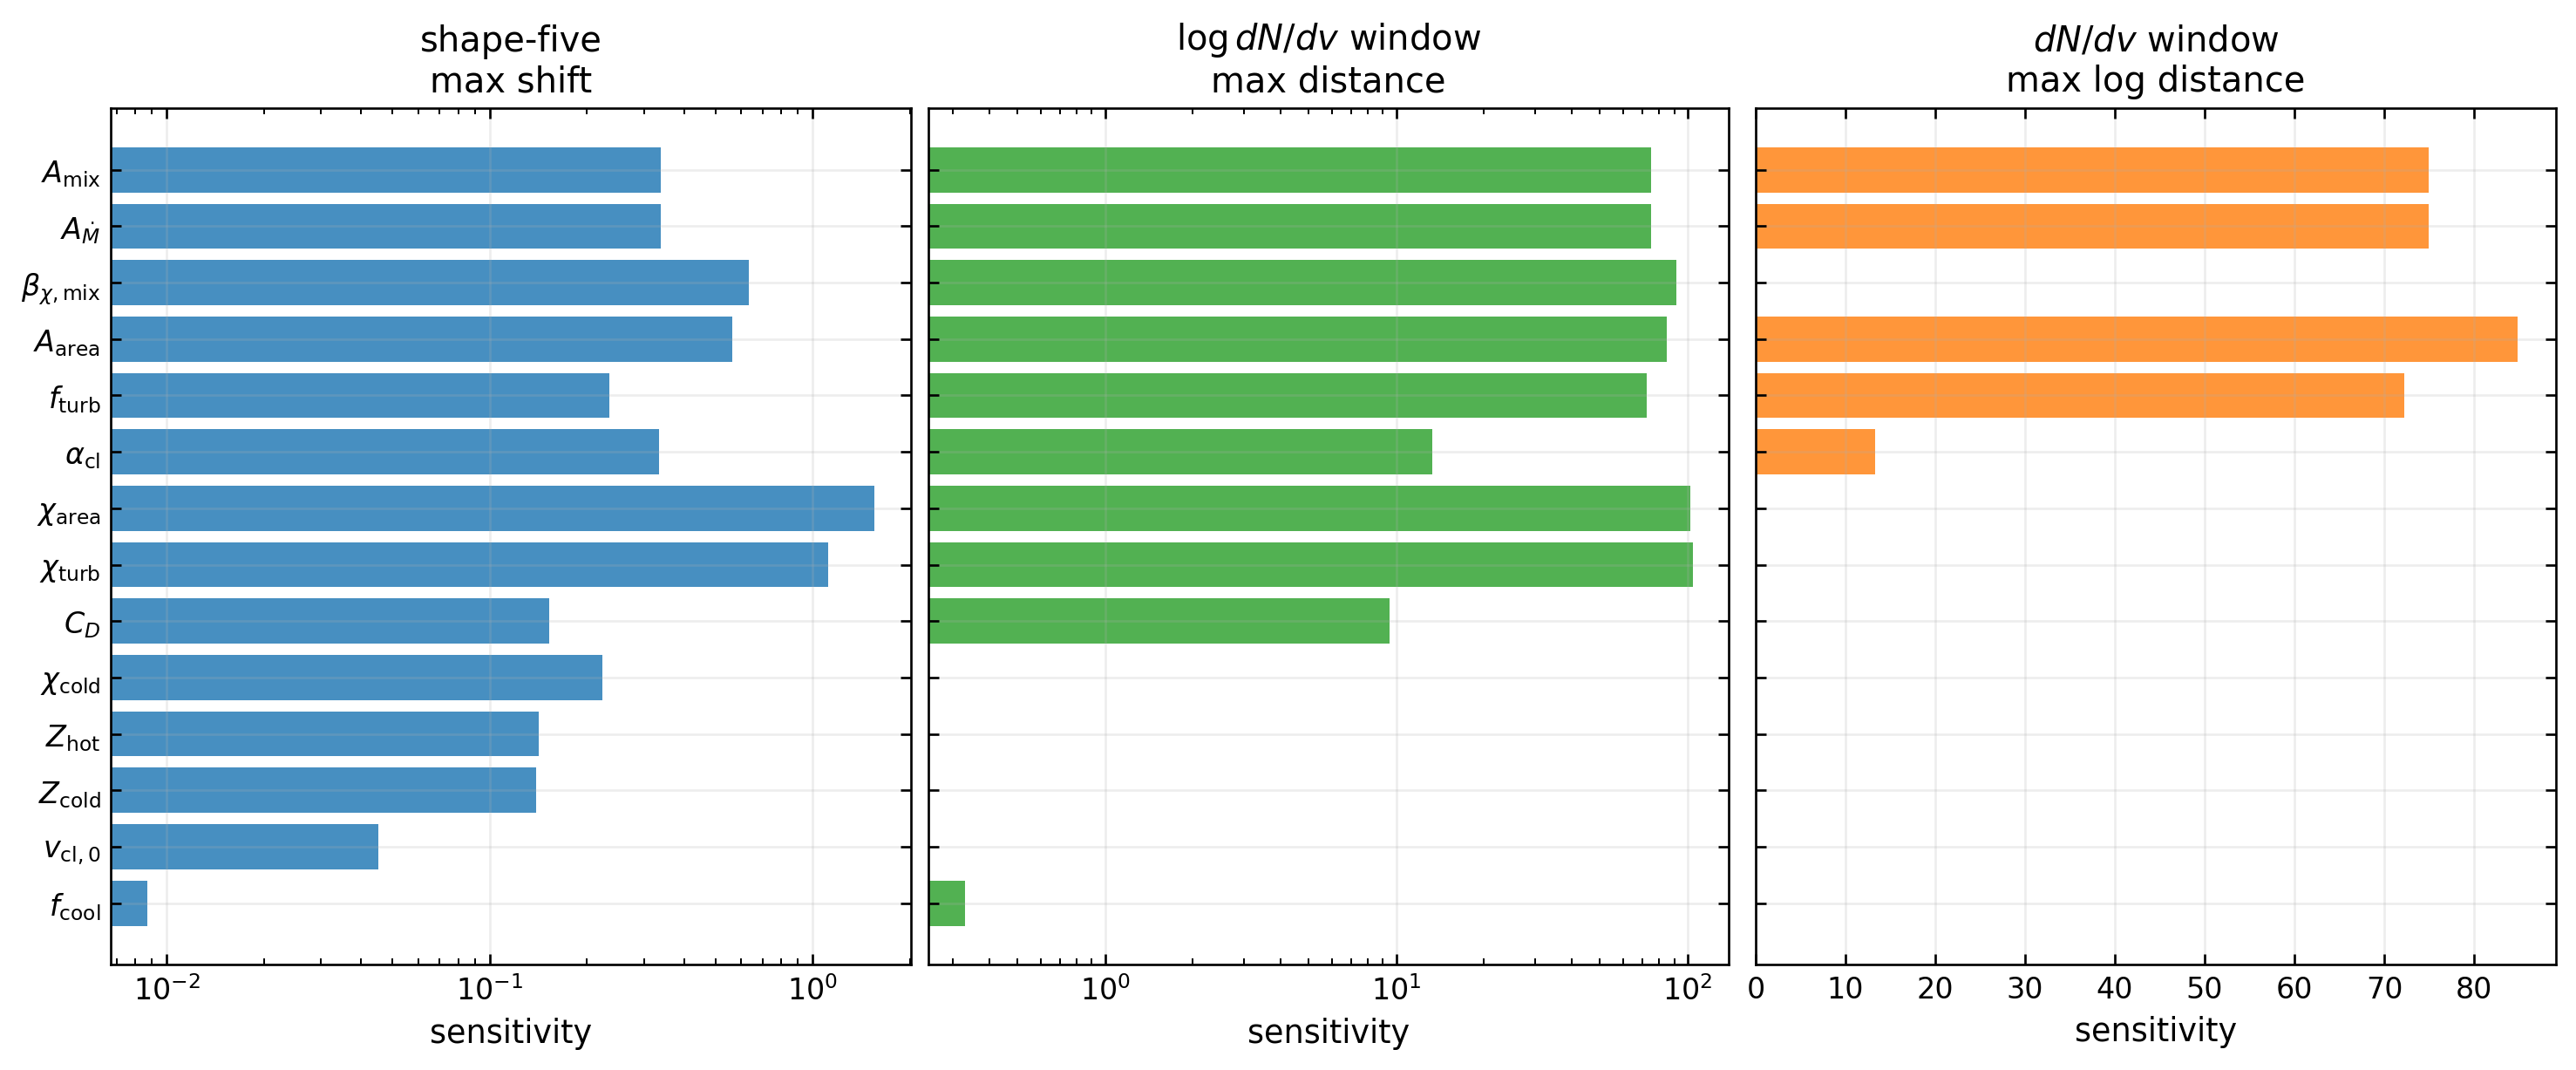
\includegraphics[width=\textwidth]{figures/trml_sensitivity_cross_case_ranking.png}
\caption{
Cross-case one-at-a-time sensitivity ranking for fixed cloud-wind and turbulent
radiative mixing-layer parameters.  The left panel shows the maximum shift in
the compact shape-five observable vector across the five synthetic truth cases.
The middle panel shows the maximum observed-window $\log dN/dv$ profile
distance for the profile-screen shortlist.  The right panel shows the analogous
linear-profile robustness check for the stable mixing-amplitude shortlist.  The
largest responses come from the $\chi$-dependent turbulent velocity and area
exponents and from effective mixing-amplitude parameters such as the
mass-exchange prefactor, geometric area factor, and $f_{\rm turb}$.  These
large shifts demonstrate that the microphysics matters for the forward model,
but they do not by themselves establish that the parameters are independently
inferable.
}
\label{fig:trml_sensitivity_cross_case_ranking}
\end{figure*}

Figure~\ref{fig:trml_sensitivity_cross_case_ranking} shows that the model is
not insensitive to the fixed microphysics.  The strongest compact-observable
responses come from the $\chi$-dependent area and turbulent-velocity exponents.
In the observed-window profile screen these same exponents can move the log
profile by tens of likelihood-scale units.  The effective amplitude-like
parameters, especially the mass-exchange prefactor, geometric area factor, and
$f_{\rm turb}$, also move both the compact summaries and the profile shape.  By
contrast, the global hot cooling multiplier is nearly inert in this reduced
screen, and the metallicity variations have lower leverage than the mixing and
turbulence parameters.

\begin{figure*}[t]
\centering
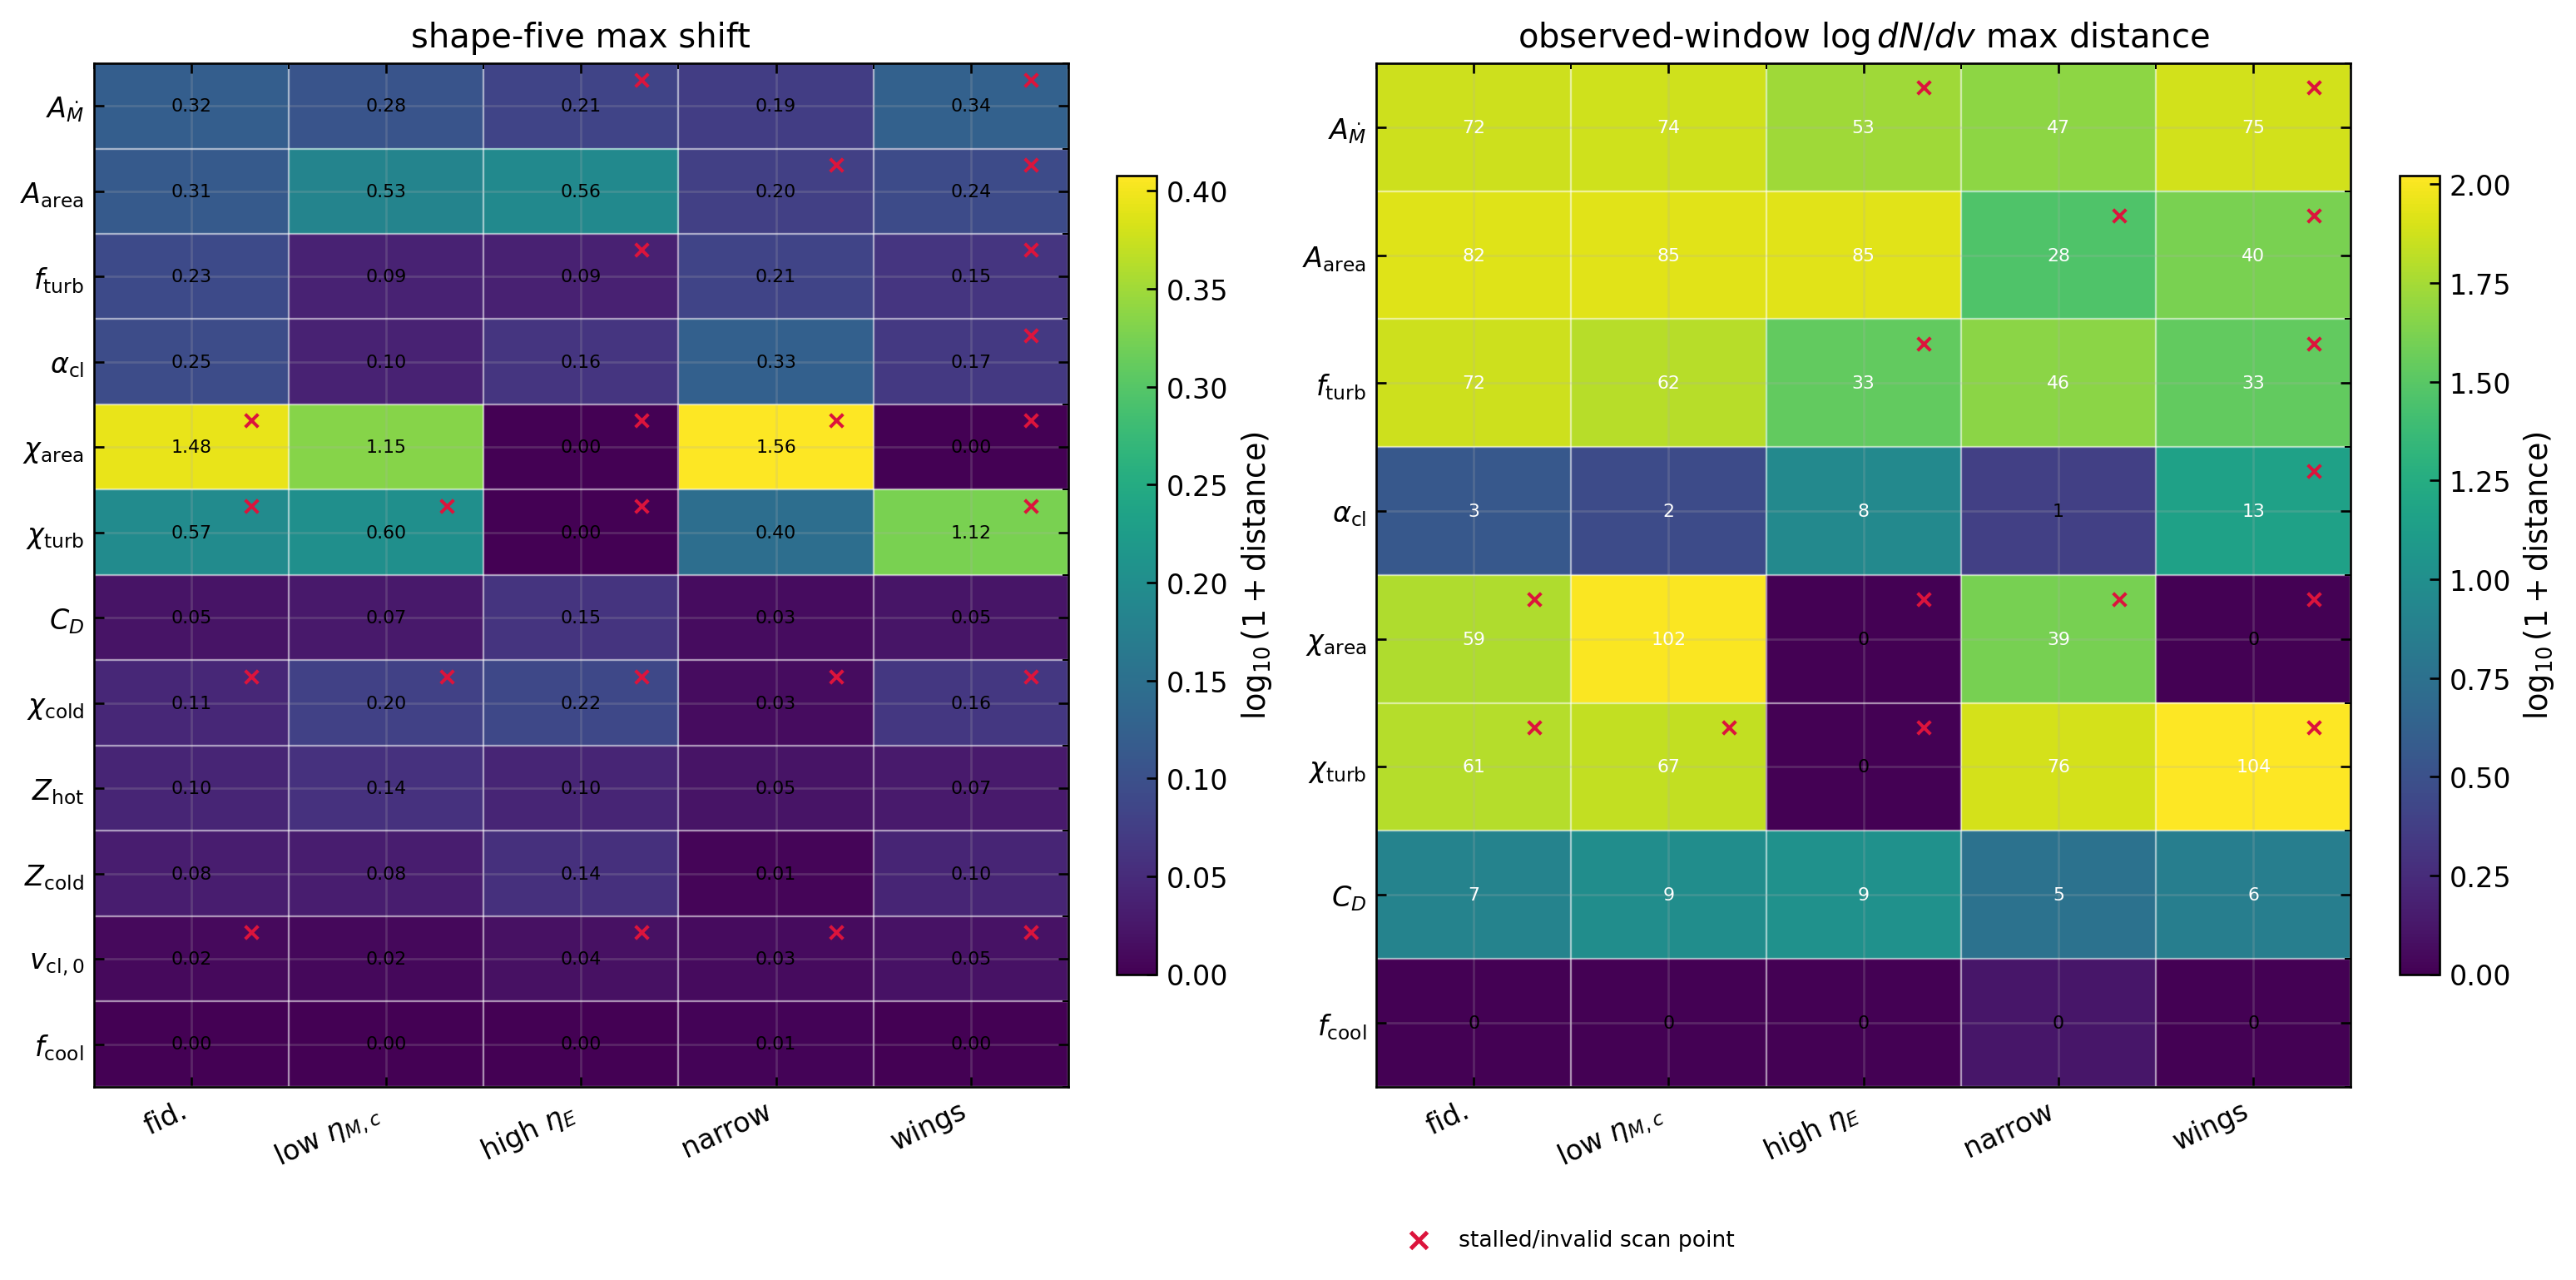
\includegraphics[width=\textwidth]{figures/trml_sensitivity_per_case_heatmap.png}
\caption{
Per-case sensitivity and validity.  The left panel shows the maximum
shape-five shift for every scanned parameter and truth case.  The right panel
shows the observed-window $\log dN/dv$ profile distance for the profile-screen
shortlist.  Cell colors use $\log_{10}(1+\mathrm{distance})$; the overplotted
numbers give the untransformed distances.  Red crosses mark truth-case and
parameter combinations for which at least one scan point stalled or became
invalid.  The heatmap shows that the conclusion is not driven solely by the
\texttt{strong\_wings} stress case: mixing-amplitude and $\chi$-exponent
directions have leverage across ordinary and high-energy cases, while the
validity problems concentrate in the same directions that most strongly alter
the wind.
}
\label{fig:trml_sensitivity_per_case_heatmap}
\end{figure*}

The important caveat is validity.  The high-leverage exponent directions often
move the model into stalled-wind regimes.  For example, increasing the cooling
area exponent or changing the turbulent-velocity exponent can cause several
truth cases to stall before the observable radius.  Stronger mixing-amplitude
settings also fail in the high-specific-energy cases: large values of the
mass-exchange prefactor or $f_{\rm turb}$ can stall
\texttt{low\_eta\_m\_high\_eta\_e} or \texttt{strong\_wings}.  This is a
physically meaningful result.  These parameter values produce winds that do not
reach the observable radius, and the stalled-wind inference policy reports them
as finite low-probability forward-model outcomes.  But they are not clean first
directions for expanded inference.

Figure~\ref{fig:trml_sensitivity_per_case_heatmap} also clarifies the role of
the \texttt{strong\_wings} case.  That case remains a deliberately difficult
stress test, but it is not the sole source of the result.  The mass-exchange
prefactor, geometric area factor, and $f_{\rm turb}$ move the observed-window
profile in the fiducial and low-cold-loading cases as well as in the high-energy
cases.  The $\chi$-dependent exponents are even more global: one sign of the
perturbation can suppress mixing enough to remove the wings, while the other
can over-couple the phases and stall the wind.  Physically, these parameters
regulate how rapidly cold material exchanges mass, momentum, and energy with
the hot flow.  When the coupling is too strong, the hot phase can lose enough
specific energy to fail before $6\,{\rm kpc}$; when it is weaker, the cool
material survives to different velocities and changes the line-profile shape.
That is exactly the microphysics we eventually want to understand, but it is
not yet a stable fourth inference coordinate.

\begin{figure*}[t]
\centering
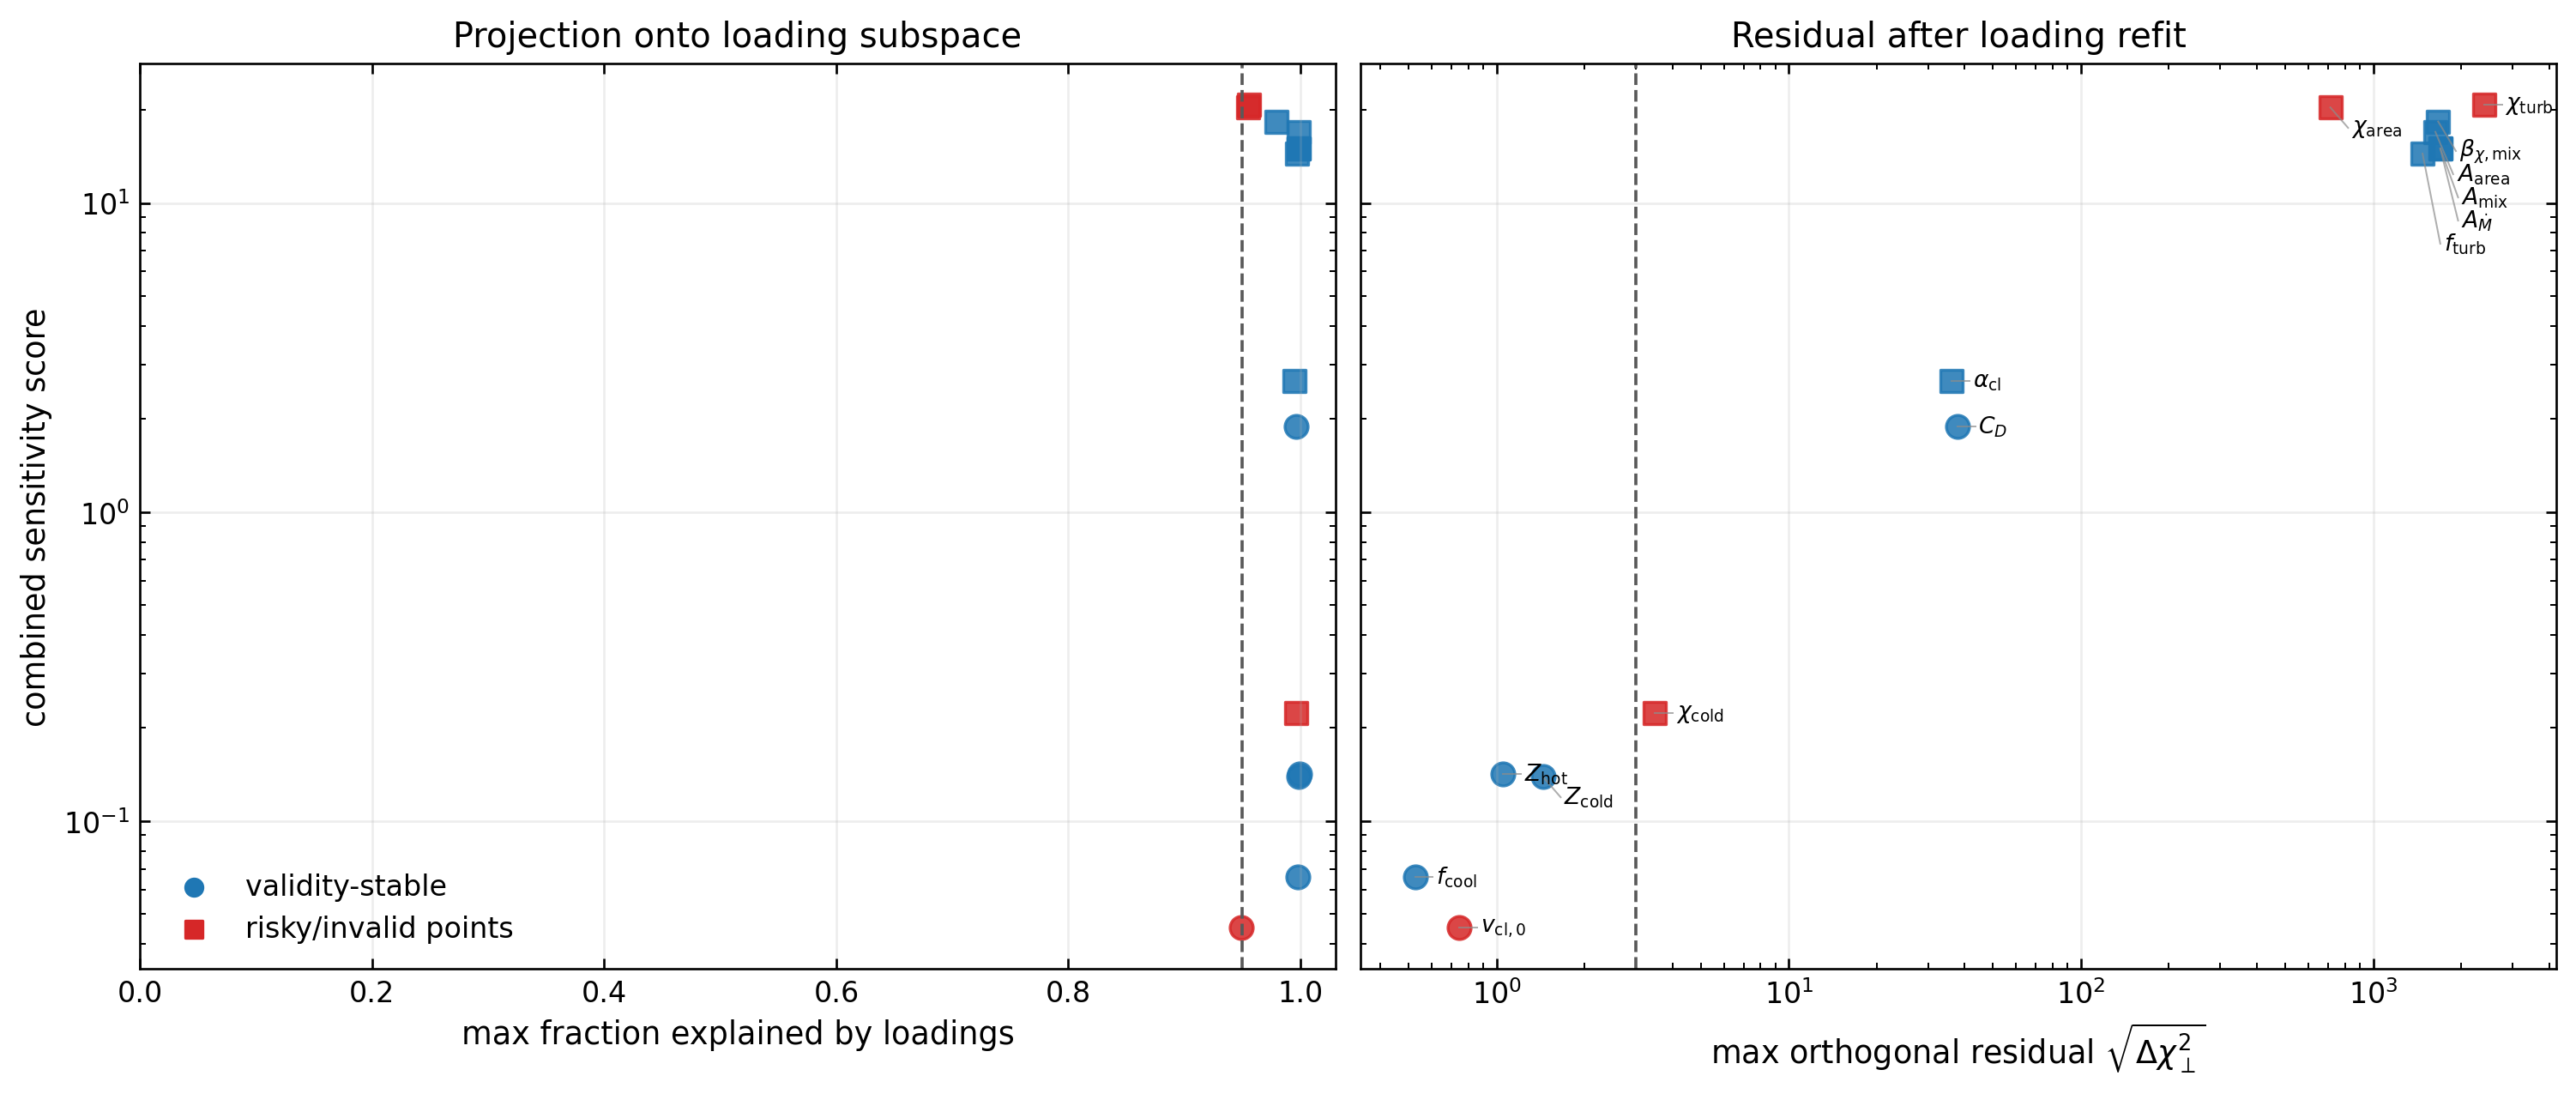
\includegraphics[width=\textwidth]{figures/trml_sensitivity_leverage_degeneracy.png}
\caption{
Observable leverage versus covariance-whitened loading-subspace projection.
The left panel shows the maximum fraction of the microphysics-induced
observable displacement that can be fit by the best linear combination of
finite-difference changes in $\eta_M$, $\eta_{M,\rm cold}$, and $\eta_E$; the
dashed line marks 0.95.  The right panel shows the remaining orthogonal
residual, $\sqrt{\Delta\chi^2_\perp}$, after that loading refit; the dashed line
marks a residual of 3.  Blue points are validity-stable across the scanned
range; red squares have repeated stalled or invalid scan points.  The
high-leverage directions are mostly loading-like in their leading response, but
their observed-window profile shifts leave large non-loading residuals under
the adopted covariance.
}
\label{fig:trml_sensitivity_leverage_degeneracy}
\end{figure*}

Figure~\ref{fig:trml_sensitivity_leverage_degeneracy} shows why this result does
not reduce to a simple yes-or-no degeneracy statement.  The leading response of
most high-leverage parameters is indeed close to the loading subspace: the
maximum explained fraction is typically $0.95$--$0.998$.  However, the profile
displacements are so large that the residual left after the best loading refit
can still be many likelihood sigma.  Thus the microphysics directions are
mostly loading-like, but not mathematically identical to loading changes.  This
is stronger evidence than the pairwise cosine test that profile data could
eventually help distinguish an effective mixing parameter from the three
loadings.

This does not mean the microphysics is unimportant.  It means that the present
observable set is not yet sufficient to infer a broad cloud-wind closure model.
The screen favors a narrow interpretation.  If an expanded parameter is tested
later, the most physically controlled first candidate is an effective mixing
amplitude, for example a multiplier on the mass-exchange prefactor.  Even that
candidate should use a restricted prior, because the high-amplitude end of the
scan produces stalled winds in the high-energy cases.  The drag coefficient is
validity-stable and has measurable profile leverage, but its overall response is
smaller than the mixing-amplitude directions and it is lower priority as a first
expansion.

The result would change in one of three ways.  First, a parameter could remain
high leverage while avoiding repeated stalled scan points over a physically
reasonable prior range.  Second, its observable displacement could become less
parallel to the loading directions, either because multiple objects are fit
jointly or because additional observables isolate the microphysics.  Third, a
restricted effective parameter such as $A_{\rm mix}$ could pass its own prior
predictive and synthetic-recovery gate.  None of those conditions is met by the
present screen.

We therefore stop short of adding a new inferred parameter at this stage.  The
Step~7 result is negative but useful: the forward model is sensitive to
cloud-wind microphysics, but the current three-parameter validation does not
support fitting a broad set of TRML closure knobs.  The next decision should
focus on a very restricted $A_{\rm mix}$ experiment with its own prior
predictive and synthetic-recovery gate, rather than a general expansion of the
closure model.

\clearpage

\section{Application to CLASSY Absorption-Line Data}
\label{sec:classy_application}

% Outline:
% - Describe the processed CLASSY inputs, including SFR, characteristic radius, circular velocity, metallicity assumptions, and observed dN/dv or moment vectors.
% - State which observable mode is chosen based on the synthetic recovery results.
% - Fit the validated baseline model, or the first expanded model if recovery supports it.
% - Present posterior constraints, degeneracies, and derived wind quantities.
% - Avoid overinterpreting parameters that remain prior dominated.

\section{Posterior Predictive Checks and Model Failures}
\label{sec:posterior_predictive}

% Outline:
% - Compare observed profiles or moments to posterior predictive bands.
% - Identify whether the model matches total column, velocity centroid, width, wings, and profile asymmetry.
% - Discuss systematic residuals as physical information, not just fit failures.
% - Connect residual patterns to possible missing physics: geometry, time variability, multiphase structure, cloud-size distribution, or line-of-sight projection.
% - State which failures are robust and which depend on covariance assumptions.

\section{Discussion}
\label{sec:discussion}

% Outline:
% - Restate the physical picture in plain language.
% - Clarify what the data constrain robustly: likely combinations of mass loading, energy loading, and cold material content.
% - Clarify what remains uncertain: detailed TRML closures and cloud-wind interaction parameters.
% - Compare with Paper 1 and explain what this paper improves: validation before interpretation.
% - Discuss implications for using absorption-line data to infer feedback physics.
% - Identify next tests: simulations, additional observables, population-level inference, and improved covariance modeling.

\section{Summary}
\label{sec:summary}

% Outline:
% - Numbered summary of the main validated results.
% - State the baseline inference status: prior predictive behavior, synthetic recovery, and real-data posterior predictive performance.
% - State whether any deeper cloud-wind parameter is identifiable enough to fit.
% - Close with the broader methodological point: physically meaningful inference requires proving recoverability before interpreting posterior constraints.

\appendix


\appendix

\section{Model Parameters and Numerical Details}
\label{app:model_details}

% Outline:
% - Provide full parameter definitions and units.
% - Summarize numerical solver settings and validity criteria.
% - Include any physics corrections relative to earlier versions of the model.

\section{Likelihoods and Covariance Models}
\label{app:likelihoods}

% Outline:
% - Define the observable vectors exactly.
% - Write the likelihood and covariance assumptions.
% - Document bin-to-bin correlation assumptions for dN/dv.

\section{Additional Validation Figures}
\label{app:additional_validation}

% Outline:
% - Reserve space for extended prior predictive atlases, recovery corner plots, and sensitivity-rank tables.
% - Keep only durable, publication-relevant figures in the manuscript source tree.


\bibliography{paper2_refs}{}
\bibliographystyle{aasjournal}

\end{document}
